\documentclass[12pt,oneside,dvipdfmx]{paper}


\usepackage{listings}
\renewcommand{\lstlistingname}{saucecode}

\lstset{%
  language={C},
  basicstyle={\small},%
  identifierstyle={\small},%
  commentstyle={\small\itshape},%
  keywordstyle={\small\bfseries},%
  ndkeywordstyle={\small},%
  stringstyle={\small\ttfamily},
  frame={tb},
  breaklines=true,
  columns=[l]{fullflexible},%
  numbers=left,%
  xrightmargin=0zw,%
  xleftmargin=3zw,%
  numberstyle={\scriptsize},%
  stepnumber=1,
  numbersep=1zw,%
  lineskip=-0.5ex%
}



% タイトル
\title{ロボコン用高出力モータードライバの開発}
\author{東出和賢}

\begin{document}
% 行間
\setlength{\baselineskip}{9truemm}

%文字間
\kanjiskip=.53zw plus 3pt minus 3pt
\xkanjiskip=.53zw plus 3pt minus 3pt

% 目次
\tableofcontents
%\newpage

% 本文
\chapter{はじめに}

\section{研究の背景}
当研究室では,毎年NHK高専ロボットコンテストに参加するためのロボット設計,及び製作を行っ
ている.過去三年間全国大会に出場しており,本校の名称が金沢工業高等専門学校である最後の年で
もあり今年度は地区大会での優勝を目標にしてて取り組んだ.

私たちは,目標達成のためには高速な移動ができるロボットが必要だと考え,ロボットの移動
方法をタイヤの二輪駆動に決め,使用するDCモータに高出力なものを使用した.
そのため,30Aでも問題ない高出力モータドライバが必要だった.そこで,伊藤研究室で
昨年作成されたITOLAB MOTORDRIVERを使用した.しかし,多くの不具合が発生したので問題解決
に向けて対策をとったものの,目標とした移動速度を下回った状態で大会に挑むこととなった.

地区大会では,初戦に一台のロボットの移動操作ができなくなるマシントラブルに遭い,地区大会
一回戦敗退という無念な結果となった.

その後,マシントラブルはモータドライバに異常があったのではという話になったが,原因を見
つけることはできなかった.
今年度のNHK高専ロボットコンテストの結果から,来年の当研究室のロボットが活躍するために,
扱いやすい高出力モータードライバが有効だと考える.

今年度のNHK高専ロボットコンテストロボットと,ロボットの足回りのモータを図\ref{fig:hontai}
と図\ref{fig:motoru}に示す.
\begin{figure}[H]
  \begin{center}
    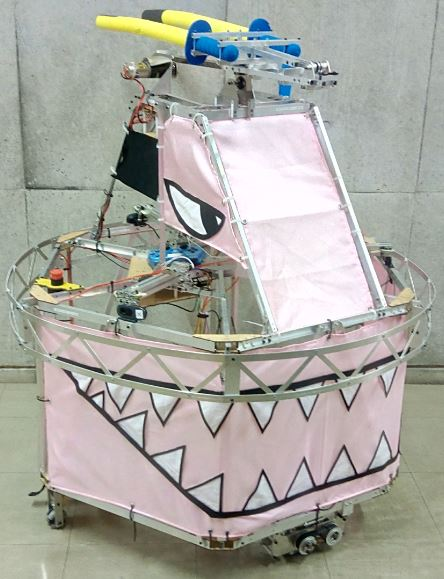
\includegraphics[width=150mm]{hontai}
    \end{center}
  \caption{ロボコンロボット}
 \label{fig:hontai}
\end{figure}
\begin{figure}[H]
  \begin{center}
    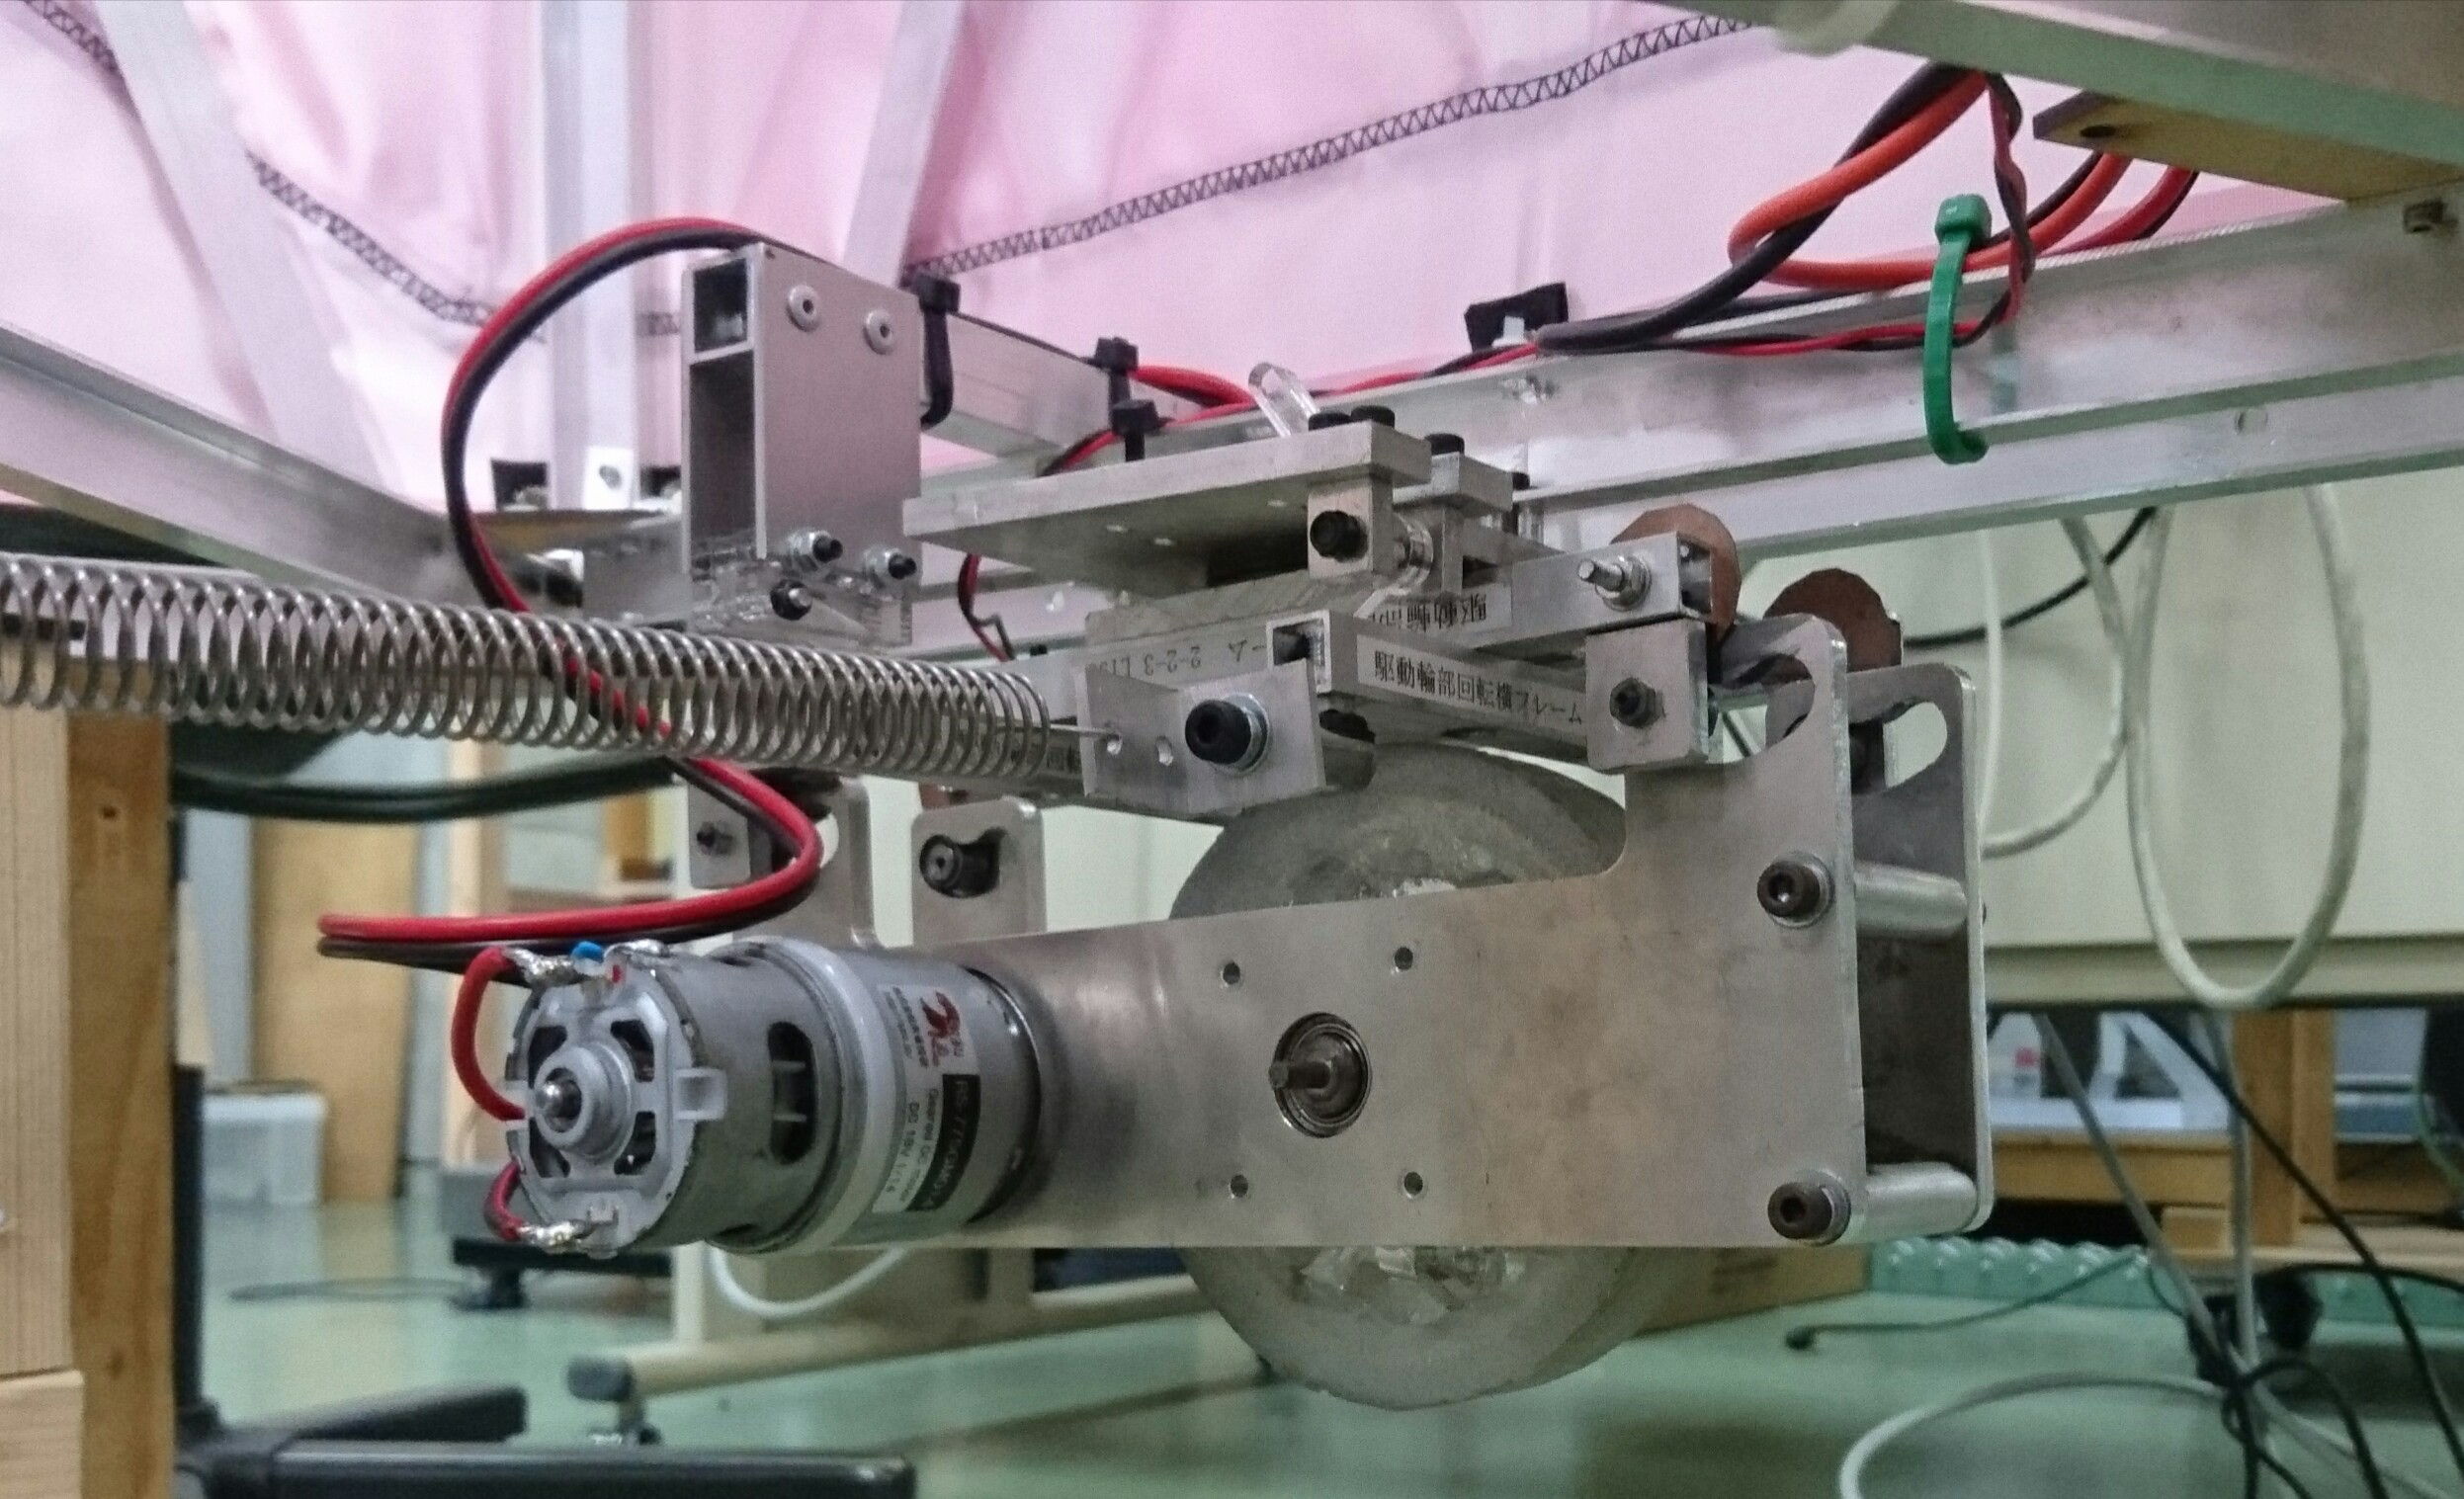
\includegraphics[width=150mm]{motoru}
    \end{center}
  \caption{足回りのモータ}
 \label{fig:motoru}
\end{figure}

\section{研究の目的}
ITOLAB MOTORDRIVERを基に,当研究室で使用できる高出力モータードライバの設計,製作を行う.

\section{本論文の構成}
1章では,本研究の背景と簡略化した概要を示す.2章では,今年のロボコンで使用した
ITOLAB MOTORDRIVERについて述べる.3章では,今回の研究で作成した高出力
モータドライバについて述べる.4章で,最後に本研究のまとめを述べる.

\chapter{ITOLAB MOTORDRIVER}

\section{ドライバの特徴}
ITOLAB MOTORDRIVERを図\ref{fig:driver}に,回路図を図\ref{fig:dra}に示す.また,
ITOLAB MOTORDRIVERの仕様を表\ref{tab:shiyou}に示す.
ロボコンでは,ロボットに使用できる部品の上限価格が設定されている.今年度の上限は30万円で
ロボットを三台作製しなければならなかった.
また,作製するロボットに自動走行させたかったので,フィードバック制御が必要だった.

そこで,エンコーダが使用でき,製作コストが安いITOLAB MOTORDRIVERを使用することにした。

\begin{figure}[H]
  \begin{center}
    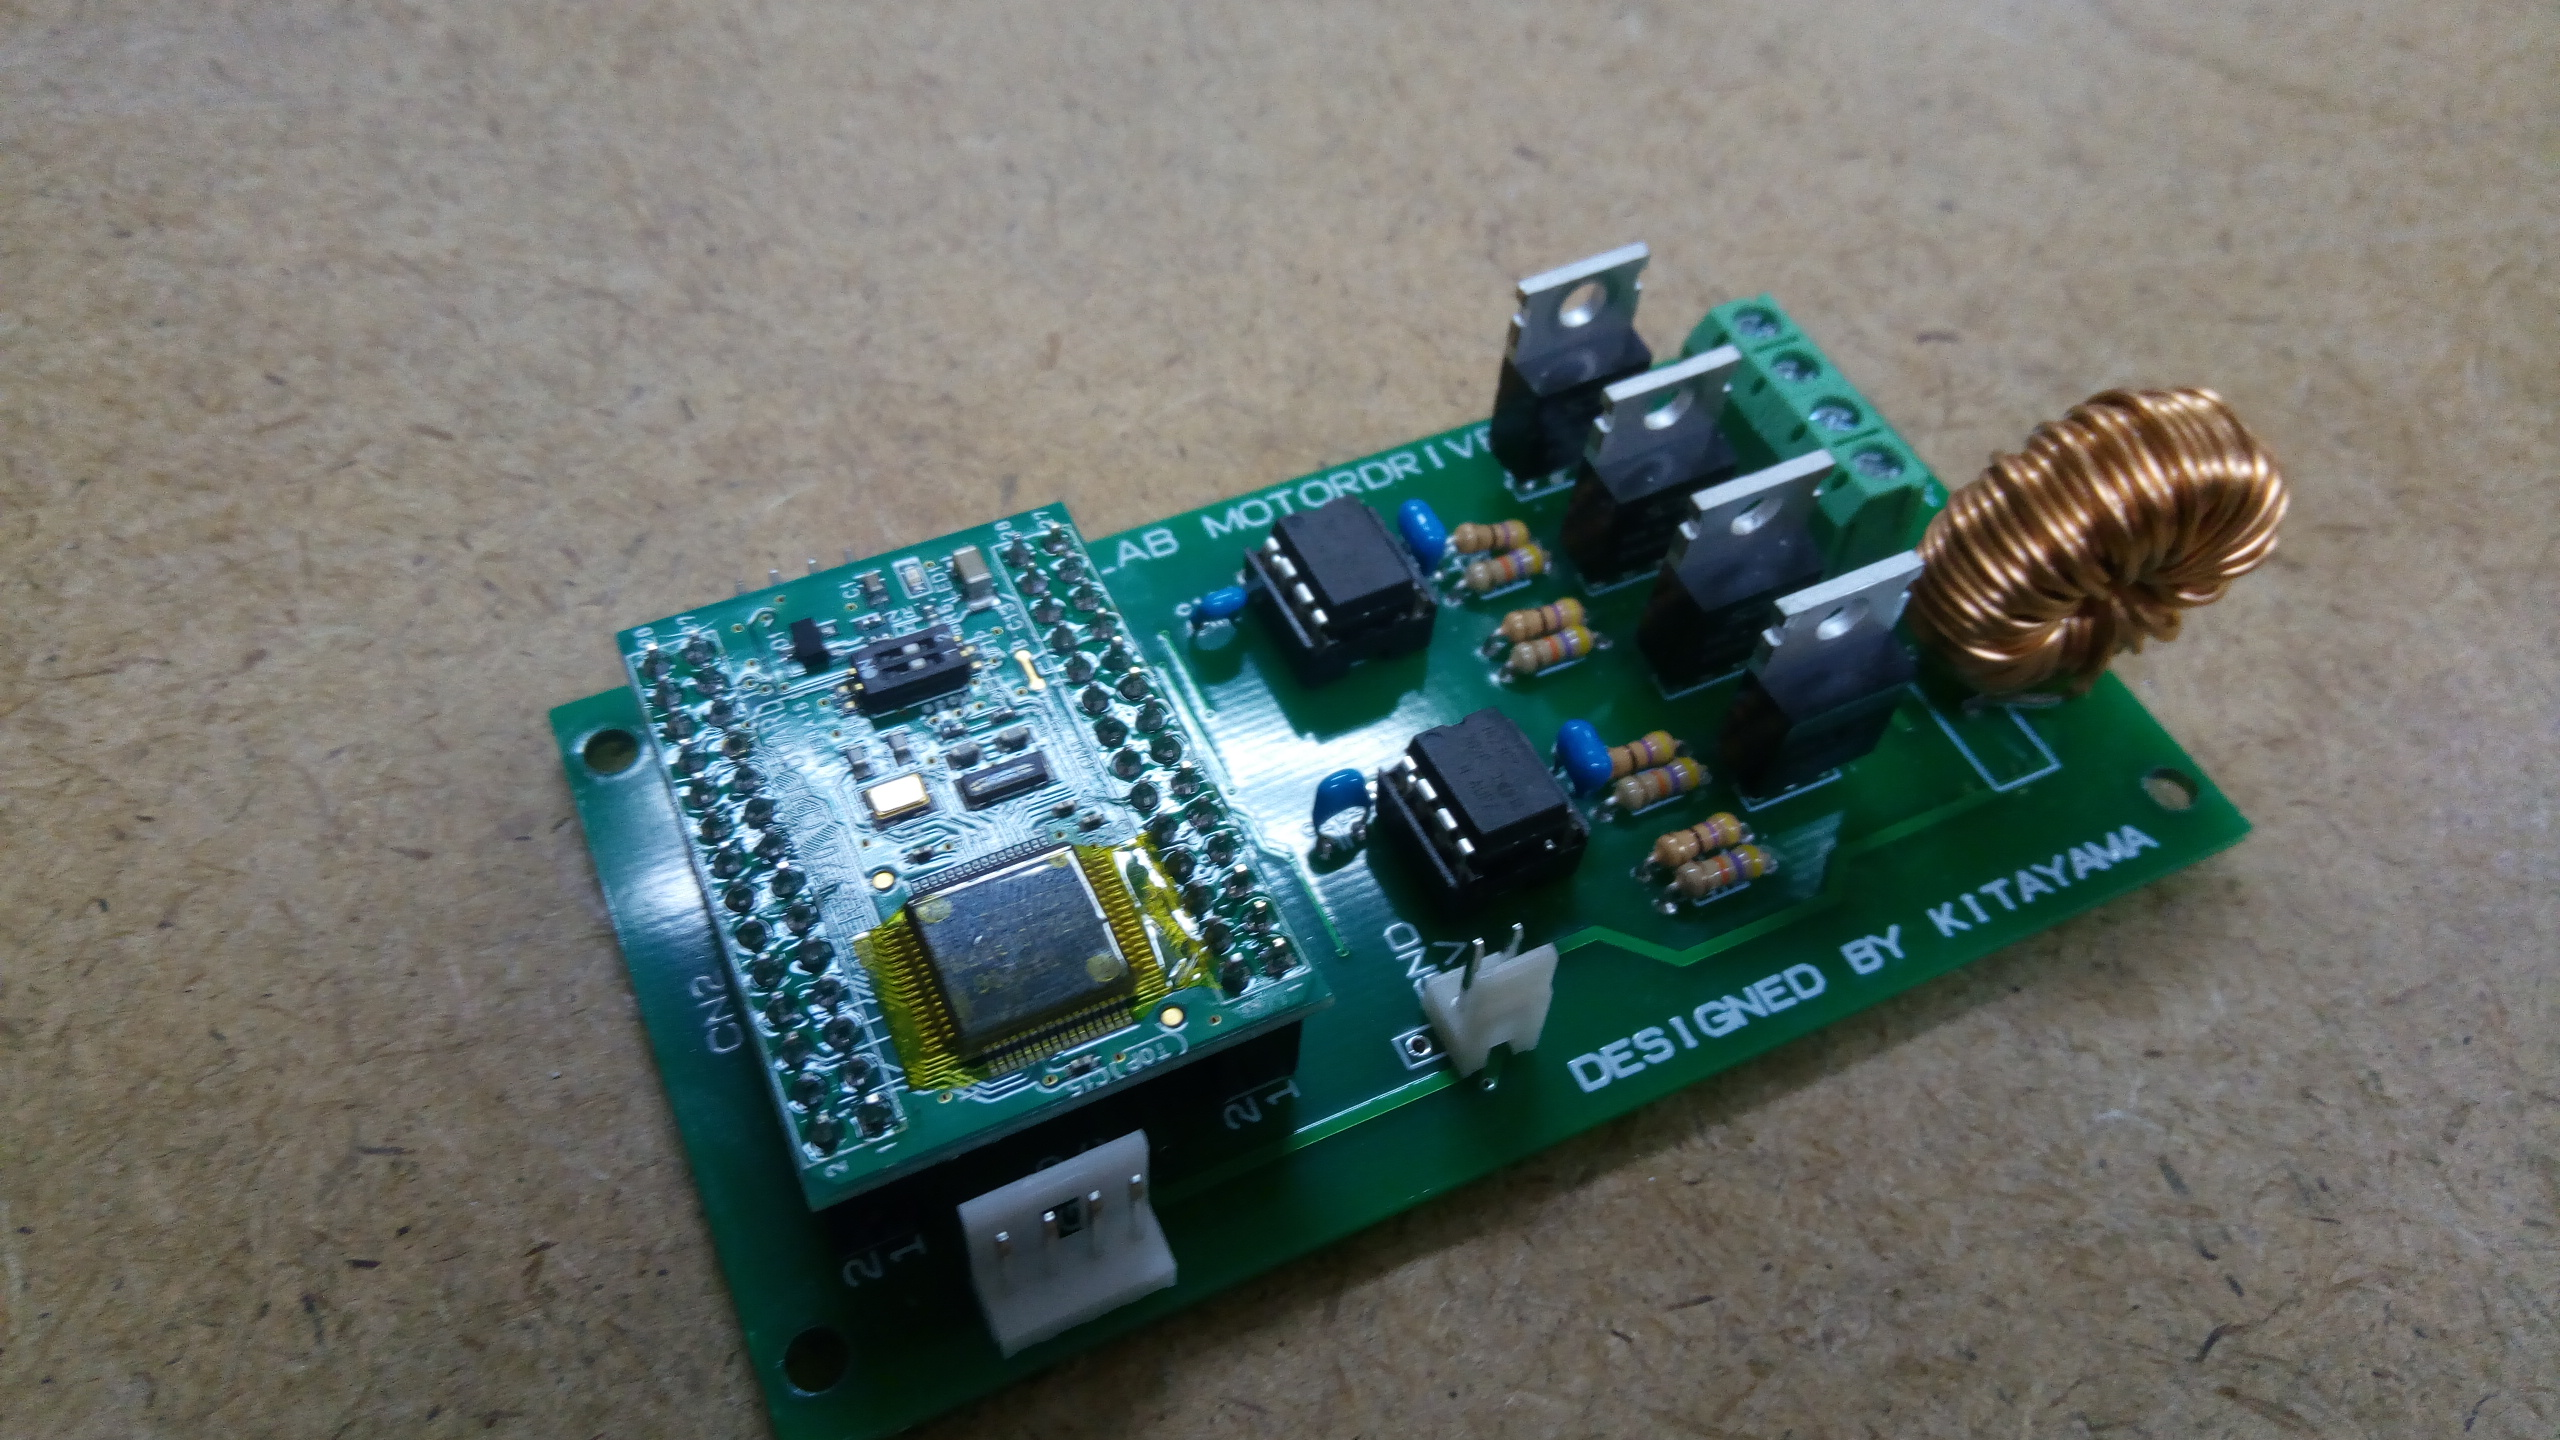
\includegraphics[width=150mm]{driver}
    \end{center}
  \caption{ITOLAB MOTORDRIVER}
 \label{fig:driver}
\end{figure}
\begin{figure}[H]
  \begin{center}
    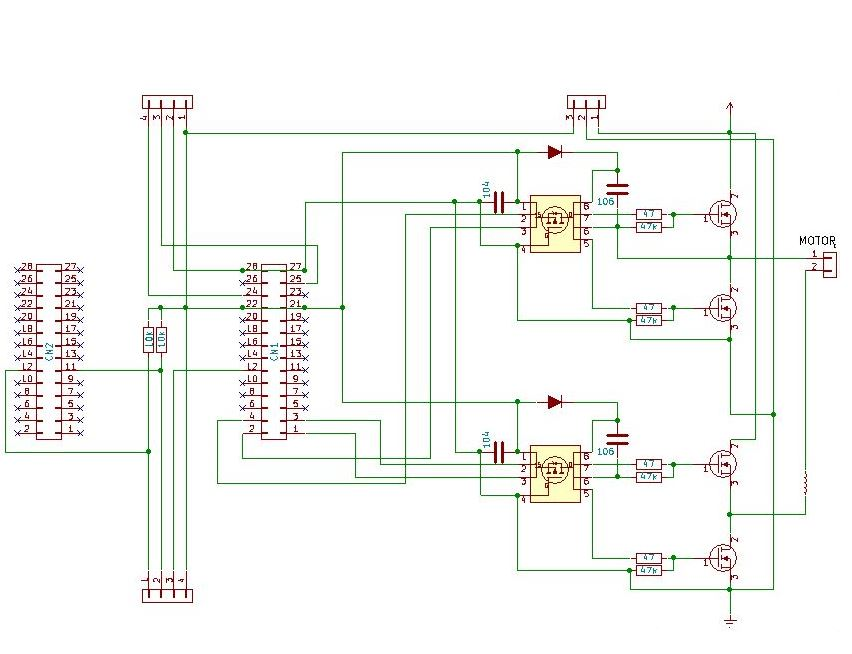
\includegraphics[width=150mm]{dra}
    \end{center}
  \caption{ITOLAB MOTORDRIVER回路図}
 \label{fig:dra}
\end{figure}
\begin{table}[htb]
\centering
\caption{ITOLAB MOTORDRIVERの仕様}
\begin{tabular}{|c|c|} \hline
使用マイコン&RX220マイコン\\ \hline
シリアル通信&RS232C\\ \hline
FET&$V_{DS}$  40V\\
   &$I_D$  80A\\ \hline
\end{tabular}
\label{tab:shiyou}
\end{table}

\section{改善点}
\subsection{発生した問題}
ロボットの動作実験を行うと,ITOLAB MOTORDRIVERに以下の問題が発生した.
\begin{itemize}
\item 急加減速時にパターンの焼損
\item 回生電流によるノイズの発生
\item FETトランジスタの高温化
\item 通信エラー
\end{itemize}
\subsubsection{パターンの焼損}
ロボットの走行実験中,ロボットを急加減速させた結果ロボット足回りから煙が上がり,
図\ref{fig:yake3}のようにモータドライバのパターンが焼損した.再現実験によりパターン
を焼損させた状態を図\ref{fig:jikkenn}に示す.
\begin{figure}[H]
  \begin{center}
    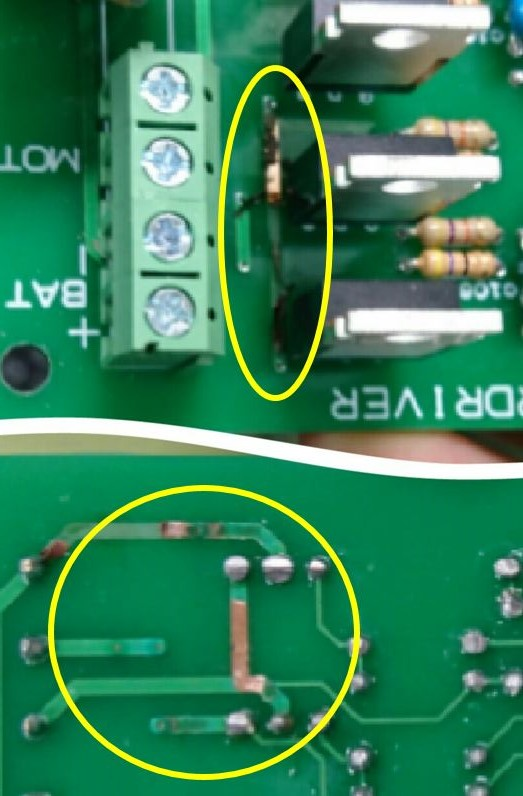
\includegraphics[width=100mm]{yake3}
    \end{center}
  \caption{パターンの焼損}
 \label{fig:yake3}
\end{figure}
\begin{figure}[H]
  \begin{center}
    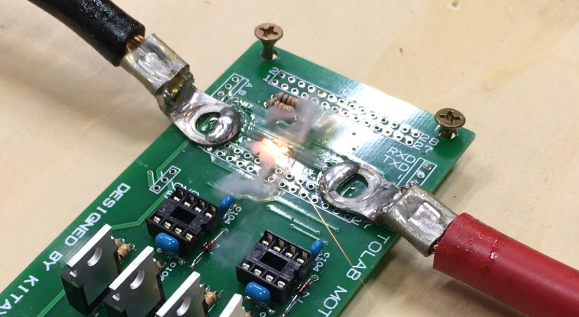
\includegraphics[width=100mm]{jikkenn}
    \end{center}
  \caption{実験によるパターンの焼損直後}
 \label{fig:jikkenn}
\end{figure}
\subsubsection{回生電流によるノイズの発生}
ロボットの走行実験中,ロボットを急加減速させた結果モータから回生電流が発生し,
ノイズとなった.
\subsubsection{FETトランジスタの高熱化}
移動速度が早いために,ロボットの前進,後進を繰り返した際電気エネルギが熱エネルギとなり,
FETトランジスタから高熱が発生された.
\subsubsection{通信エラー}
回生電流で発生したノイズによって,RS232C通信にノイズが乗り急停止時にロボットが暴走した.

\subsection{問題に対しての改善}
これらを解決するために,以下の対策を講じた.
改善後のITOLAB MOTORDRIVERを図\ref{fig:shin_driver}に,ロボットに取り付けた
ITOLAB MOTORDRIVERを図\ref{fig:robotuke}に示す.
\begin{itemize}
\item 電流制限プログラムの作成
\item 回生ダイオードの取り付け
\item FETトランジスタにヒートシンクの取り付け
\item 通信エラー確認用のLEDの取り付け
\end{itemize}
\subsubsection{電流制限プログラムの作成}
急加減速をするとパターンの焼損するので,プログラムで加減速を緩やかにして最高速度を
下げた.
\subsubsection{回生ダイオードの取り付け}
図\ref{fig:kai}の回生ダイオードを取り付けることで,モータから発生する回生電流から基板
を守り,ノイズを防ぐ.
\begin{figure}[H]
  \begin{center}
    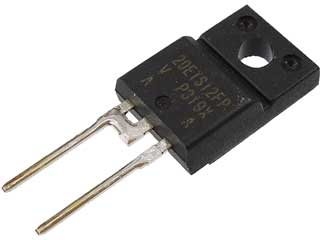
\includegraphics[width=50mm]{kai}
    \end{center}
  \caption{回生ダイオード}
 \label{fig:kai}
\end{figure}
\subsubsection{FETトランジスタにヒートシンクの取り付け}
ロボット操作によってFETで発生した熱を,図\ref{fig:hi-to}のヒートシンクで放熱,冷却する.
\begin{figure}[H]
  \begin{center}
    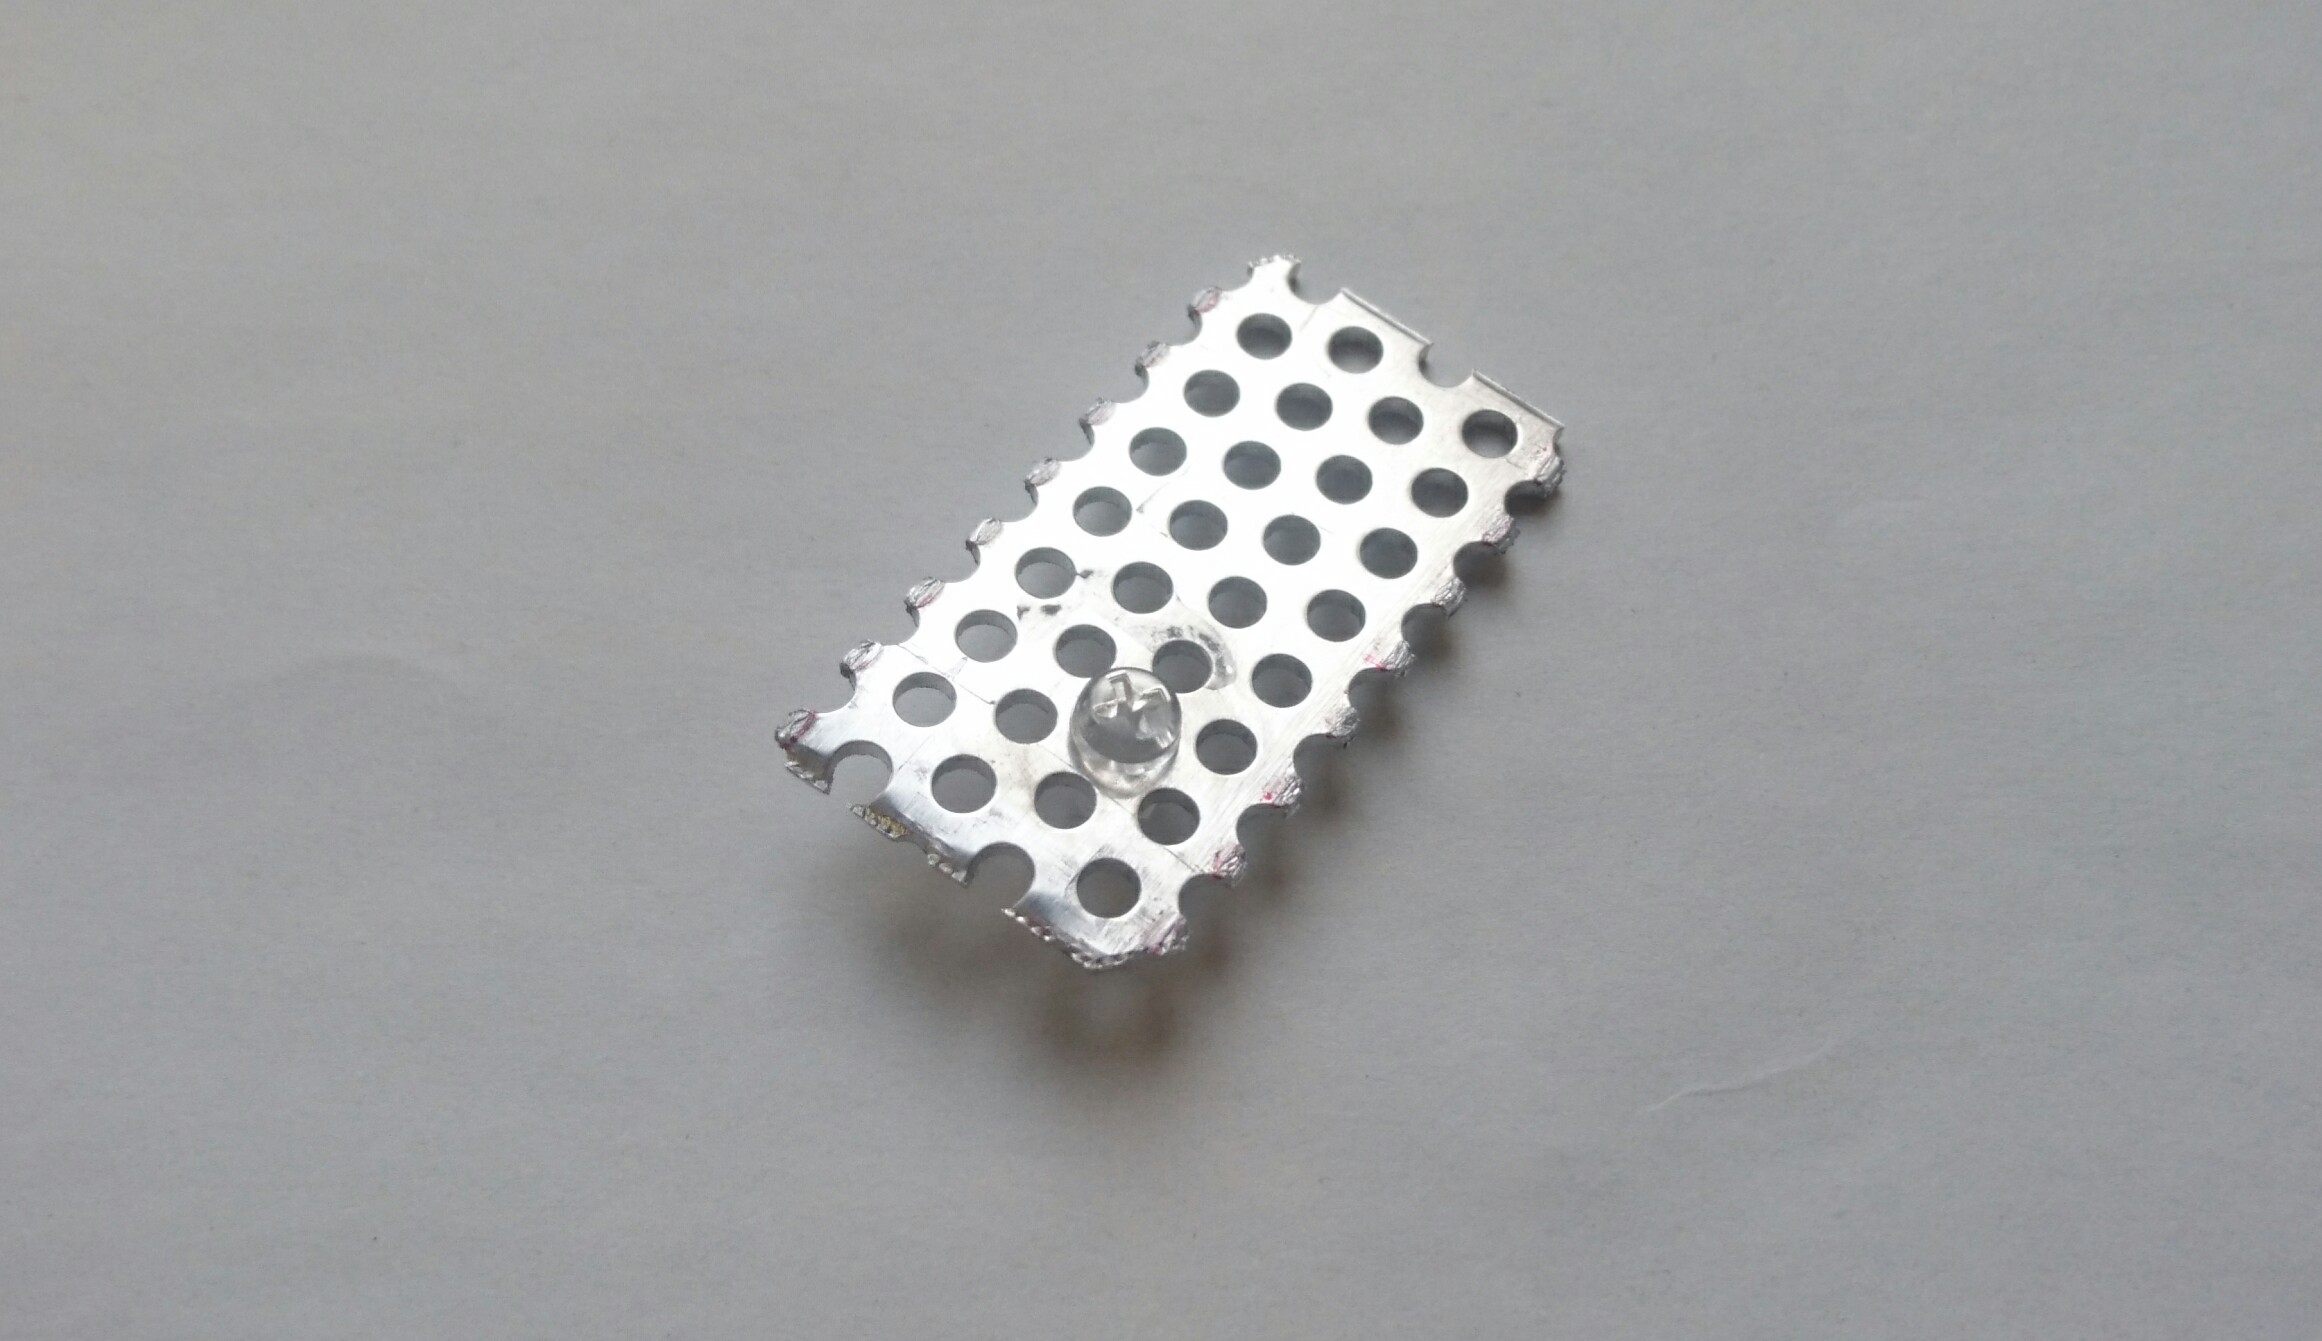
\includegraphics[width=50mm]{hi-to}
    \end{center}
  \caption{ヒートシンク}
 \label{fig:hi-to}
\end{figure}
\subsubsection{通信エラー確認用のLEDの取り付け}
RX220マイコンに図\ref{fig:led}のLEDを取り付け,通信エラーが発生した時に光るように
プログラムした.
\begin{figure}[H]
  \begin{center}
    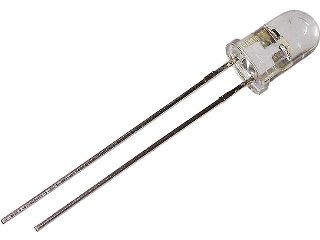
\includegraphics[width=50mm]{led}
    \end{center}
  \caption{5mm 砲弾型LED}
 \label{fig:led}
\end{figure}
\begin{figure}[H]
  \begin{center}
    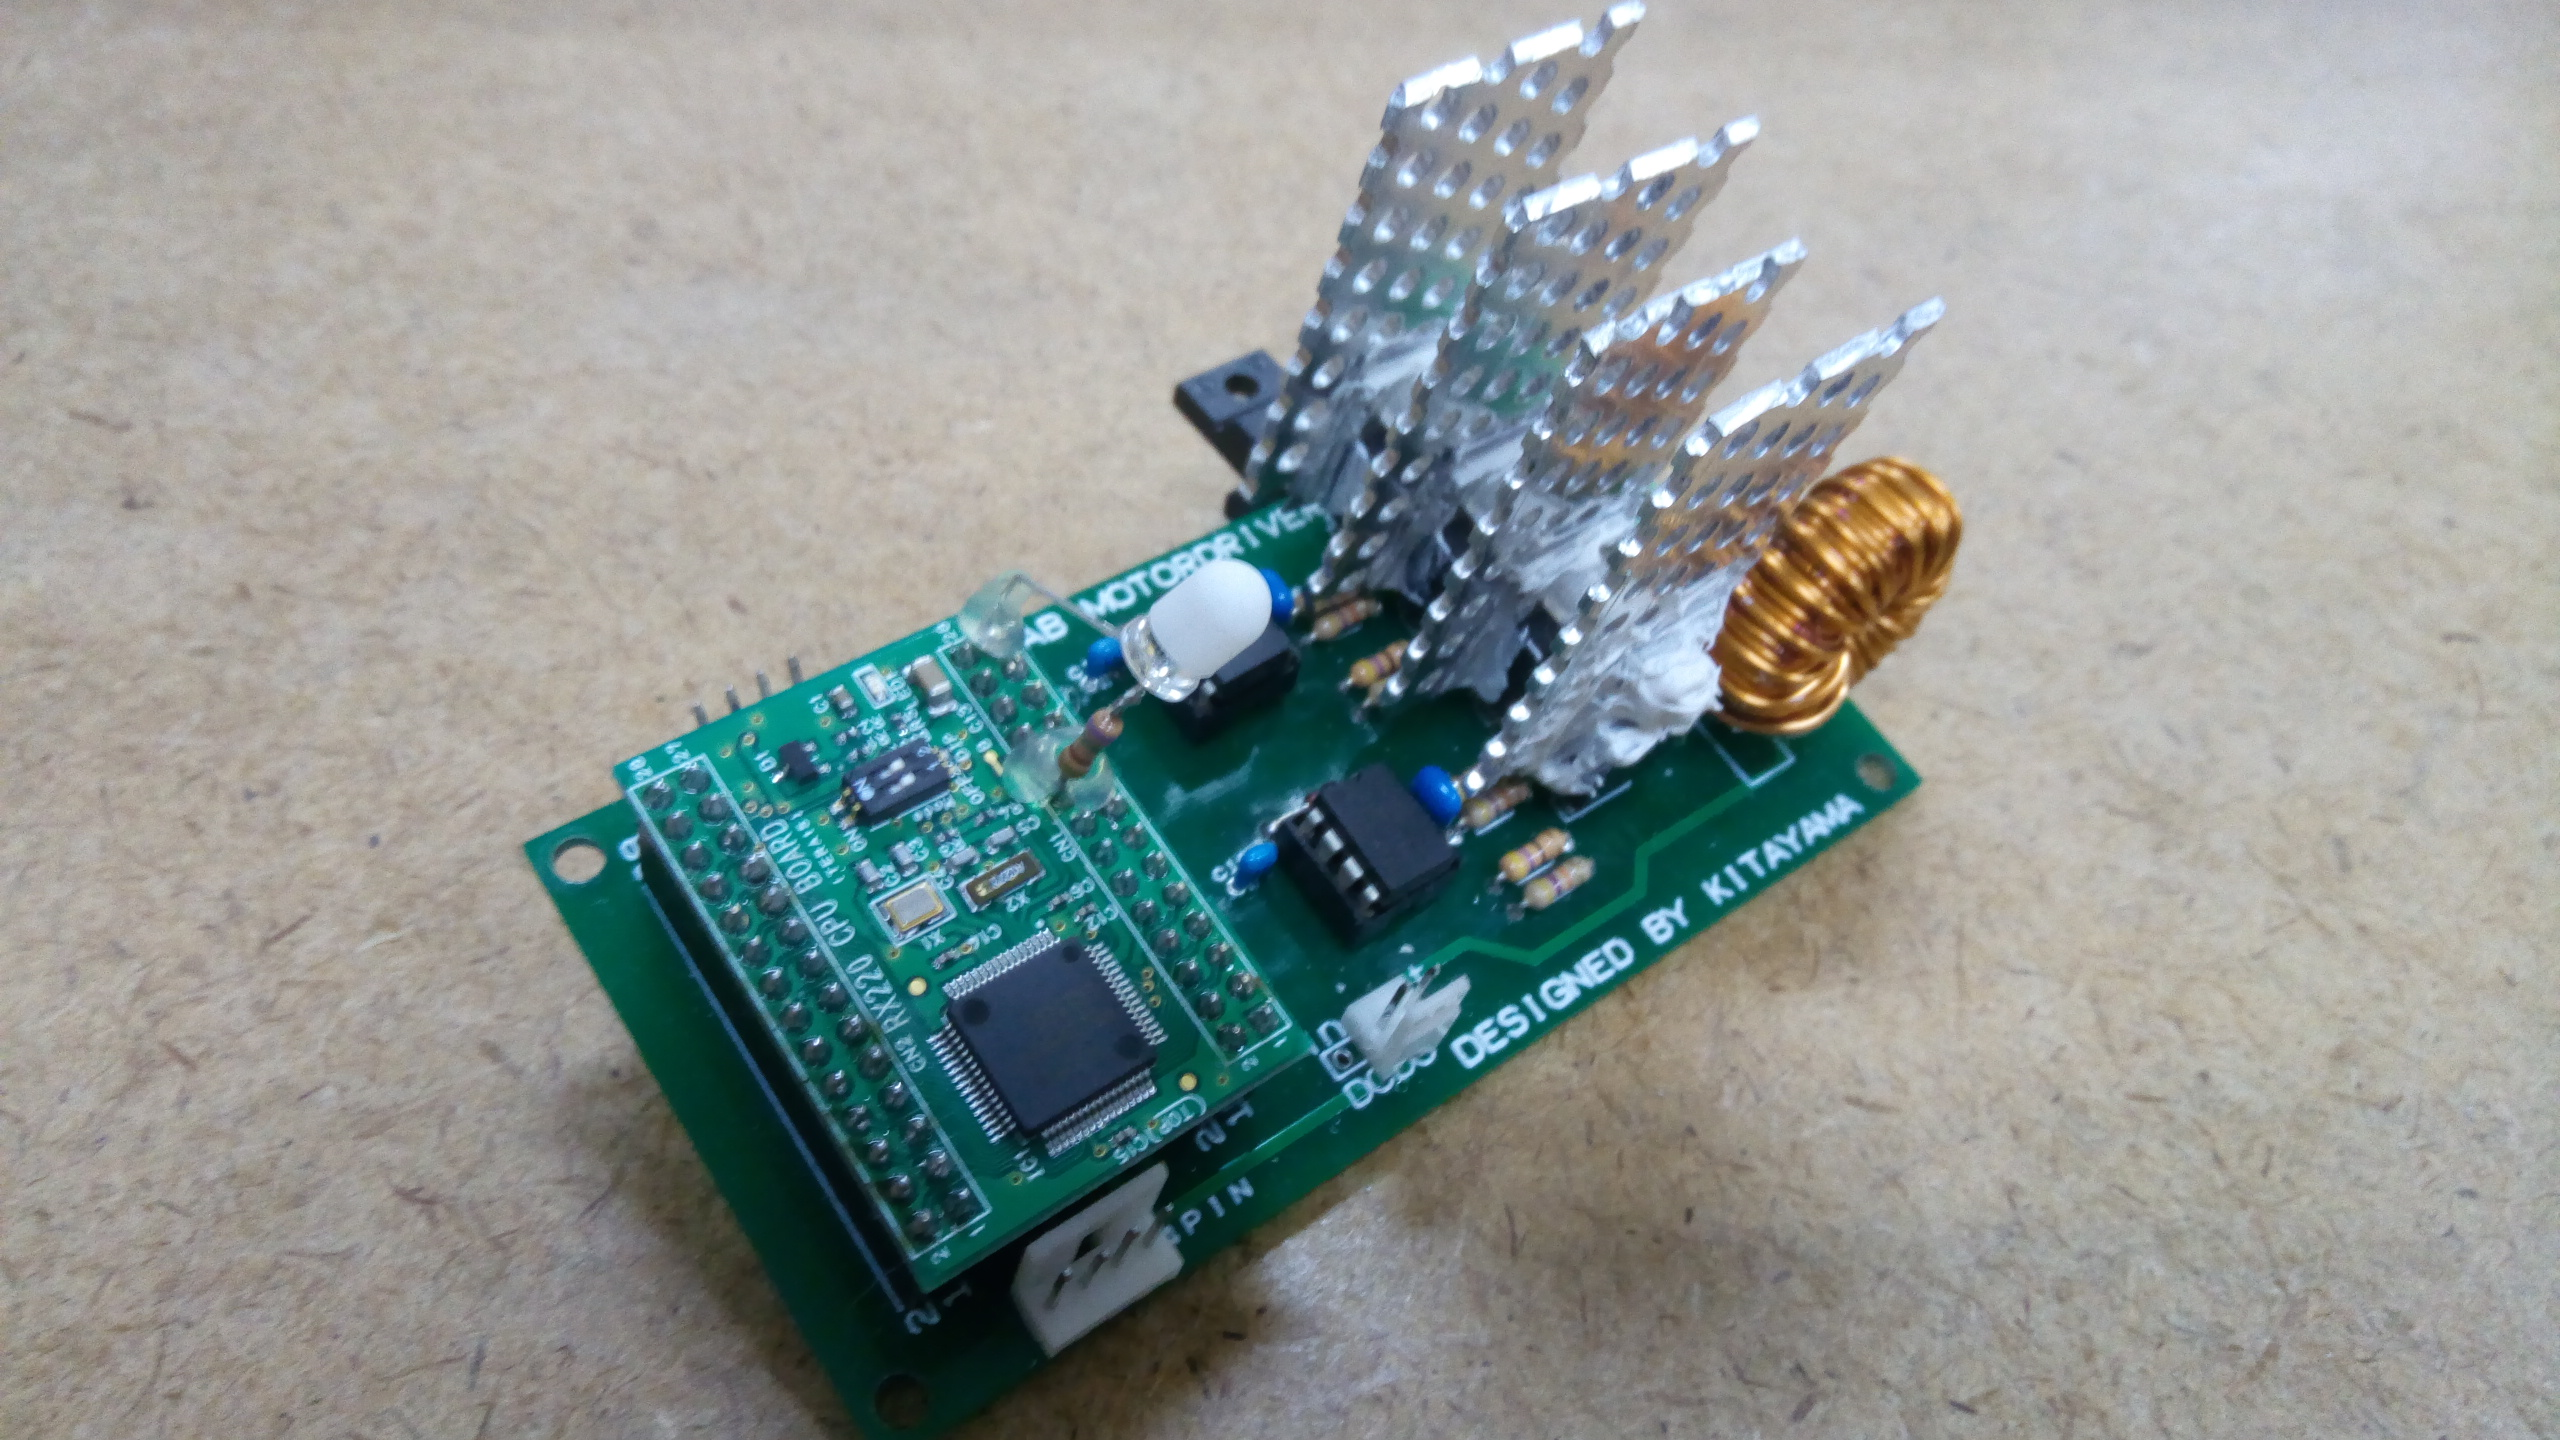
\includegraphics[width=150mm]{shin_driver}
    \end{center}
  \caption{改善後のITOLAB MOTORDRIVER}
 \label{fig:shin_driver}
\end{figure}
\begin{figure}[H]
  \begin{center}
    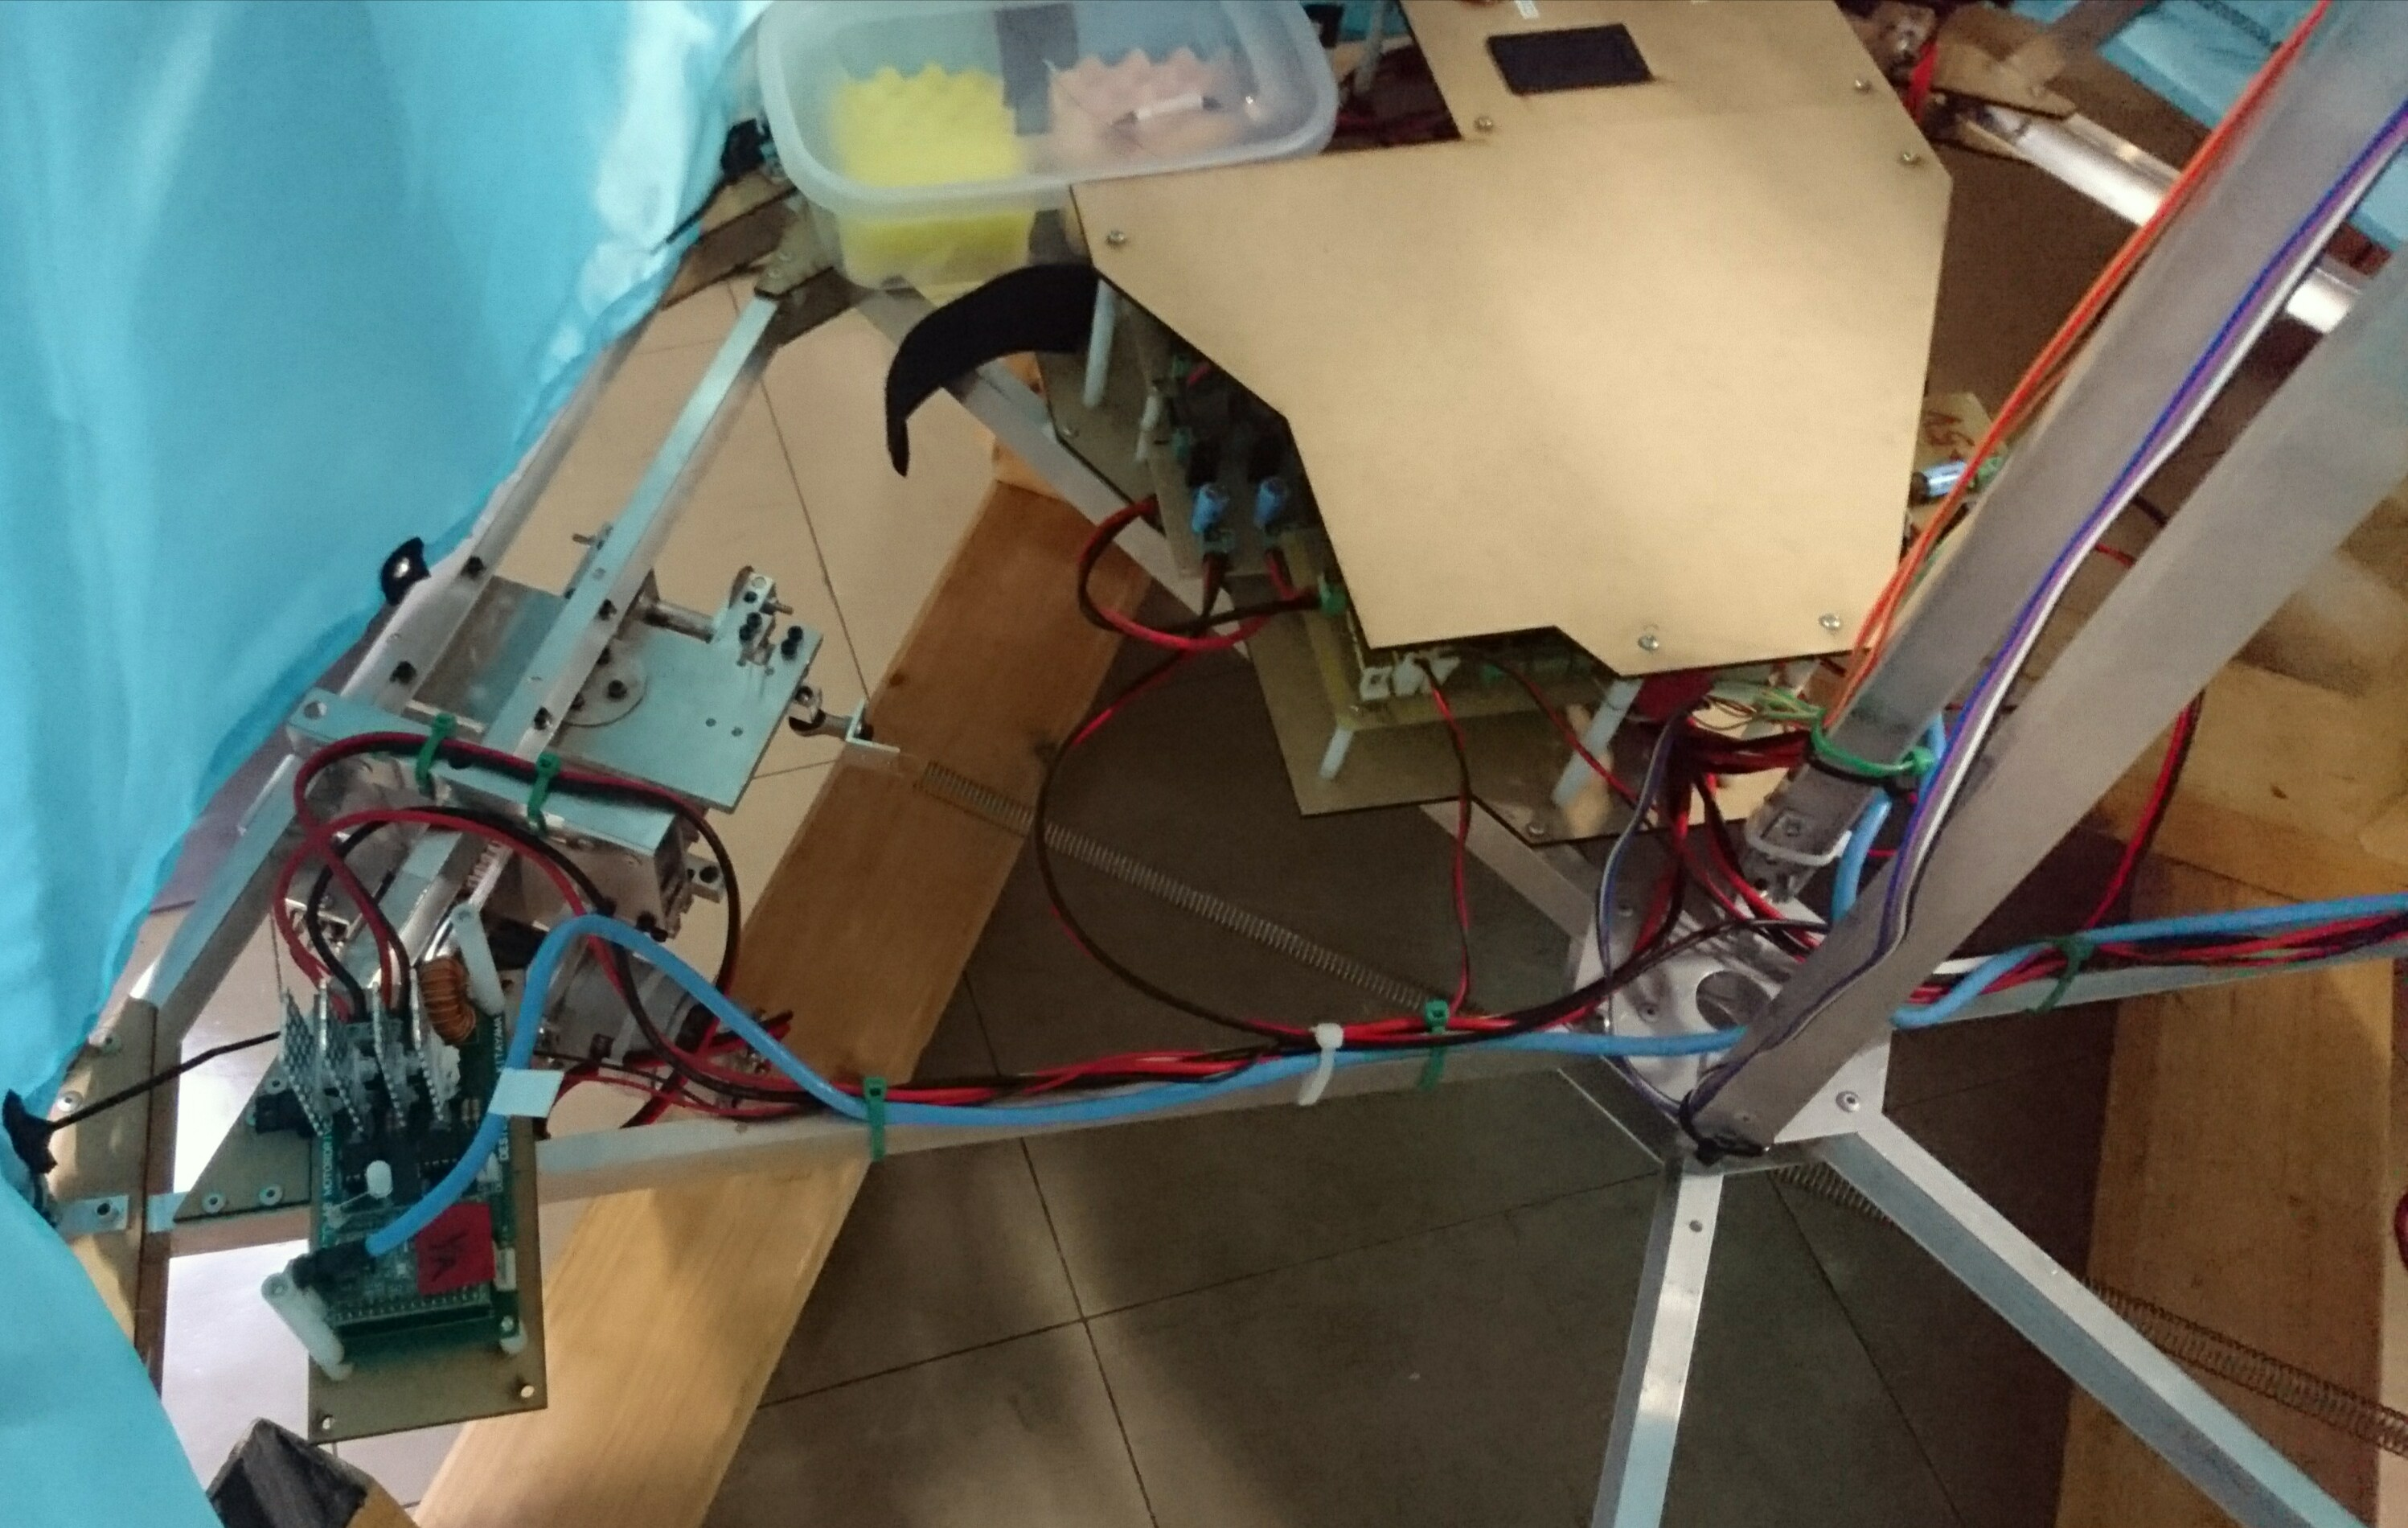
\includegraphics[width=150mm]{robotuke}
    \end{center}
  \caption{ロボットに取り付けたITOLAB MOTORDRIVER}
 \label{fig:robotuke}
\end{figure}

\section{ITOLAB MOTORDRIVER使用結果}
ロボットの最大移動速度を5.83m/sにするために,回転数を1114rpmに設定した.しかし,
電流制限プログラムを入れたために,目標の1114rpmに達せず,700rpmまでとなった.

また,地区大会時に図\ref{fig:teishi}のように1台のロボットのモータが動作
しなくなった.試合後には動作したので,原因を調べたが原因を発見できず,モータドライバ
の不具合も発見できなかった.
\begin{figure}[H]
  \begin{center}
    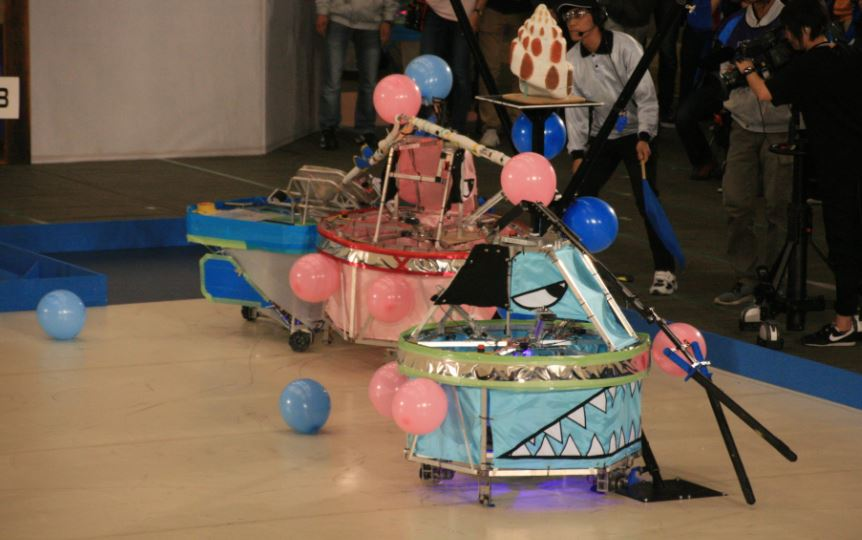
\includegraphics[width=150mm]{teishi}
    \end{center}
  \caption{停止したロボット}
 \label{fig:teishi}
\end{figure}


\chapter{新高出力モータドライバ}

\section{要求機能}
ロボコンで使用するバッテリーは,最大電圧14.8V,最大電流178Aで,モータは最大電流130Aである.
このことから,ITOLAB MOTORDRIVERでバッテリー,モータの性能を最大まで発揮できていない
ことが分かる.
これを考慮した上で,
先に述べた不具合箇所を修正,改良した高出力モータドライバを製作した.
\begin{itemize}
\item 大電流が流れるパターン幅の拡張,GNDのベタ化
\item FETヒートシンク,回生ダイオードの標準搭載
\item FET用温度センサの取り付け
\item モータに流れる電流を確認するための電流センサの取り付け
\item エラー,通信を確認するための汎用LEDの取り付け
\item 制御用マイコンのリセットスイッチ,実験などに使用できる汎用スイッチの搭載
\item ノイズの影響を受けやすいRS232通信から,影響の受けにくい作動伝送を用いた
RS485通信への変更
\end{itemize}


\section{構成}
新高出力モータードライバのシステムブロック図を図\ref{fig:shisutemu}に示す.
また,新モータドライバの仕様書を表\ref{tab:shinshiyou}に示す.付録CにRXマイコンと
各部品との接続を示した.
\begin{figure}[H]
  \begin{center}
    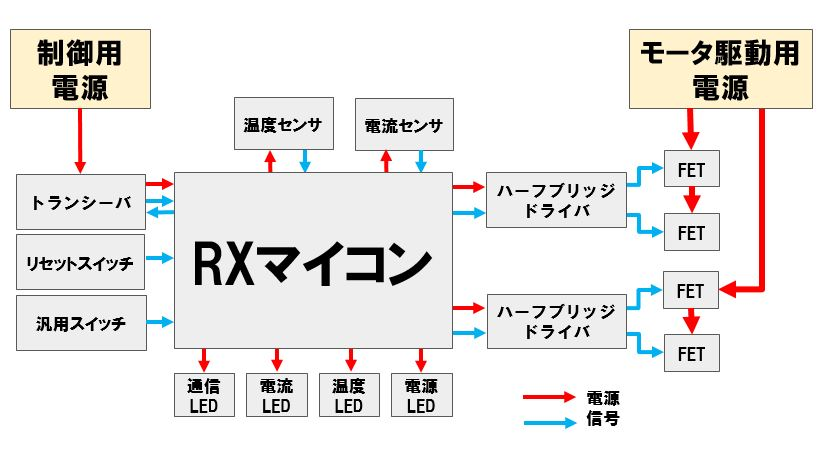
\includegraphics[width=150mm]{shisutemu}
    \end{center}
  \caption{システムブロック図}
 \label{fig:shisutemu}
\end{figure}
\begin{table}[htb]
\centering
\caption{新モータドライバの仕様書}
\begin{tabular}{|c|c|} \hline
使用マイコン&RX220マイコン\\ \hline
シリアル通信&RS485\\ \hline
FET&$V_{DS}$  40V\\
   &$I_D$  80A  \\ \hline
温度センサ&動作温度 -40~125℃ \\
&動作電圧 3.1~5.5V \\ \hline
電流センサ&動作温度 -40~150℃\\
&作動電圧 3.3~5.5V \\
&検出電流 0~100A \\ \hline
最大定格電圧&40V\\ \hline
最大定格電流&80A\\ \hline
\end{tabular}
\label{tab:shinshiyou}
\end{table}

\section{回路図・アートワーク図}
ロボコン用高出力モータードライバの回路図,アートワーク図をそれぞれ図\ref{fig:kairozu}
,図\ref{fig:a-towa-ku}に示す.また,基板の3Dビューアを図\ref{fig:3Dbyu-a}に示す.
回路図,アートワークの作成は,回路図とアートワークが連動しているKiCadを用いた.
回路図は,ITOLAB MOTORDRIVERの回路図を作成した後に,新たな部品を接続した.

アートワークは,大電流の流れる可能性のあるパターン幅を,1.0mmから5.0mmに変更した.
パターン幅と電流許容量は比例しているので,電流の許容量は5倍になる.
また,裏面はGNDのベタ化を行った.
\begin{figure}[H]
\begin{center}
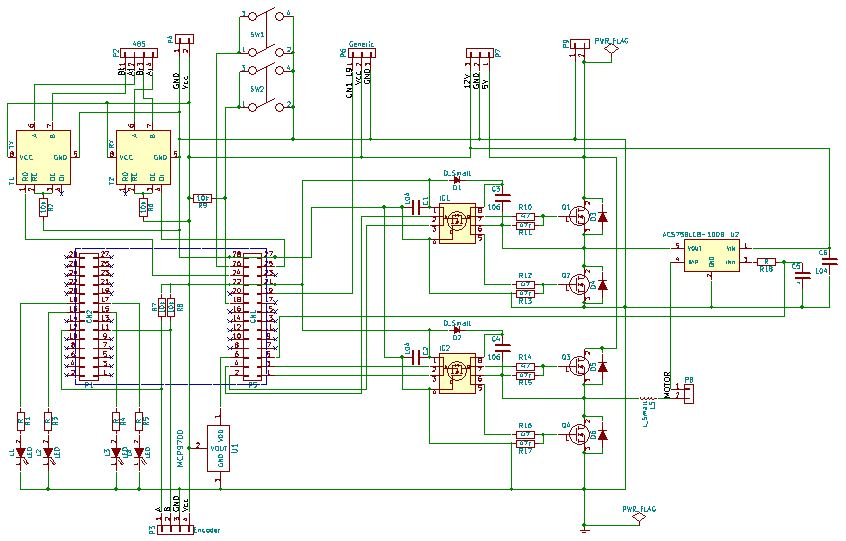
\includegraphics[width=150mm]{kairozu}
\end{center}
\caption{回路図}
\label{fig:kairozu}
\end{figure}
\begin{figure}[H]
\begin{center}
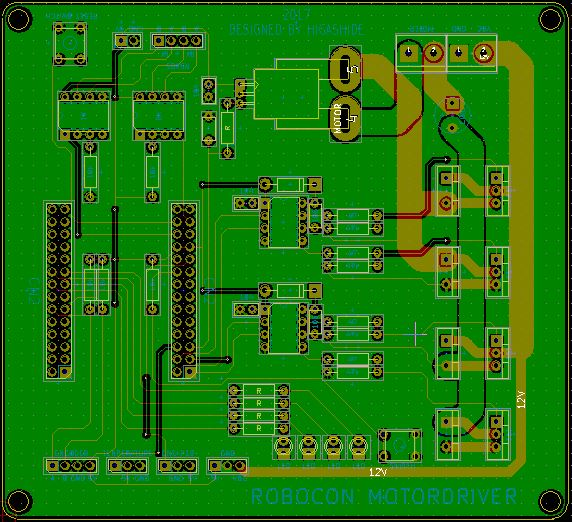
\includegraphics[width=150mm]{a-towa-ku}
\end{center}
\caption{アートワーク図}
\label{fig:a-towa-ku}
\end{figure}
\begin{figure}[H]
\begin{center}
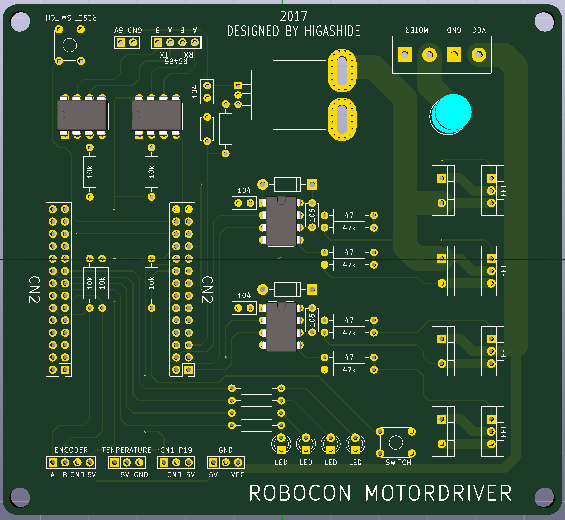
\includegraphics[width=150mm]{3Dbyu-a}
\end{center}
\caption{3Dビューア}
\label{fig:3Dbyu-a}
\end{figure}

\section{完成品}
ロボコン用高出力モータドライバの完成品を図\ref{fig:kansei}に,組み付けたものを図\ref{fig:kankumi}に示す.
基板の製作は,Fusion PCBに依頼した.
\begin{figure}[H]
\begin{center}
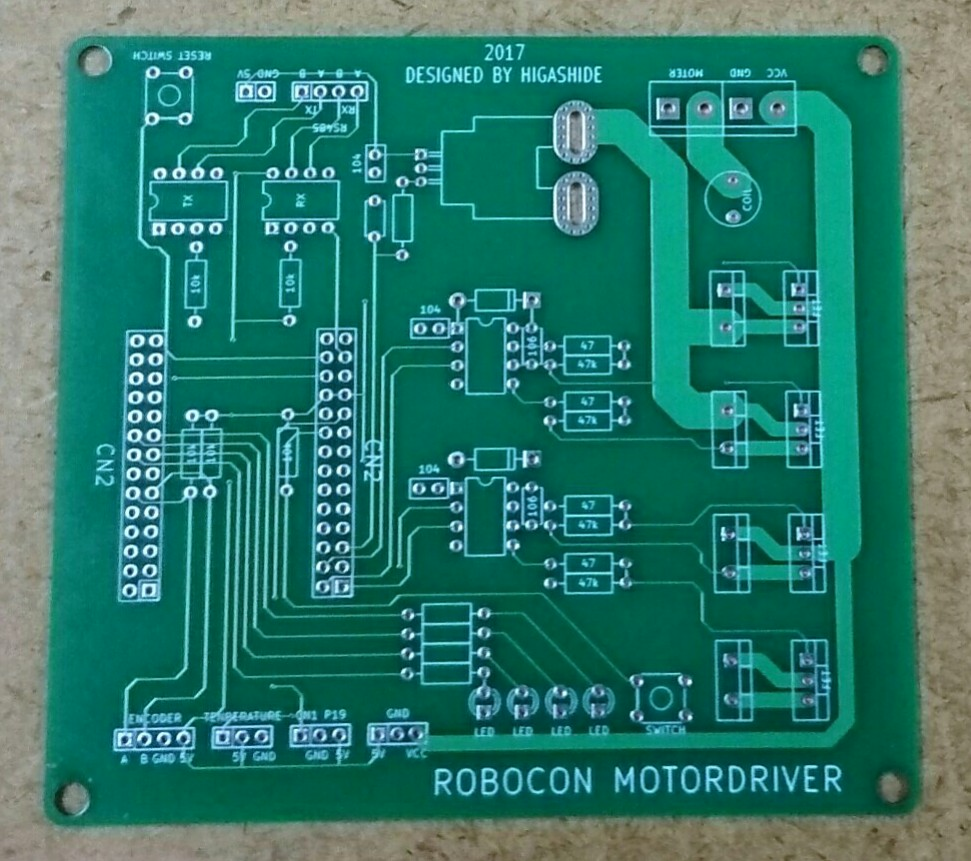
\includegraphics[width=150mm]{kansei}
\end{center}
\caption{完成品}
\label{fig:kansei}
\end{figure}
\begin{figure}[H]
\begin{center}
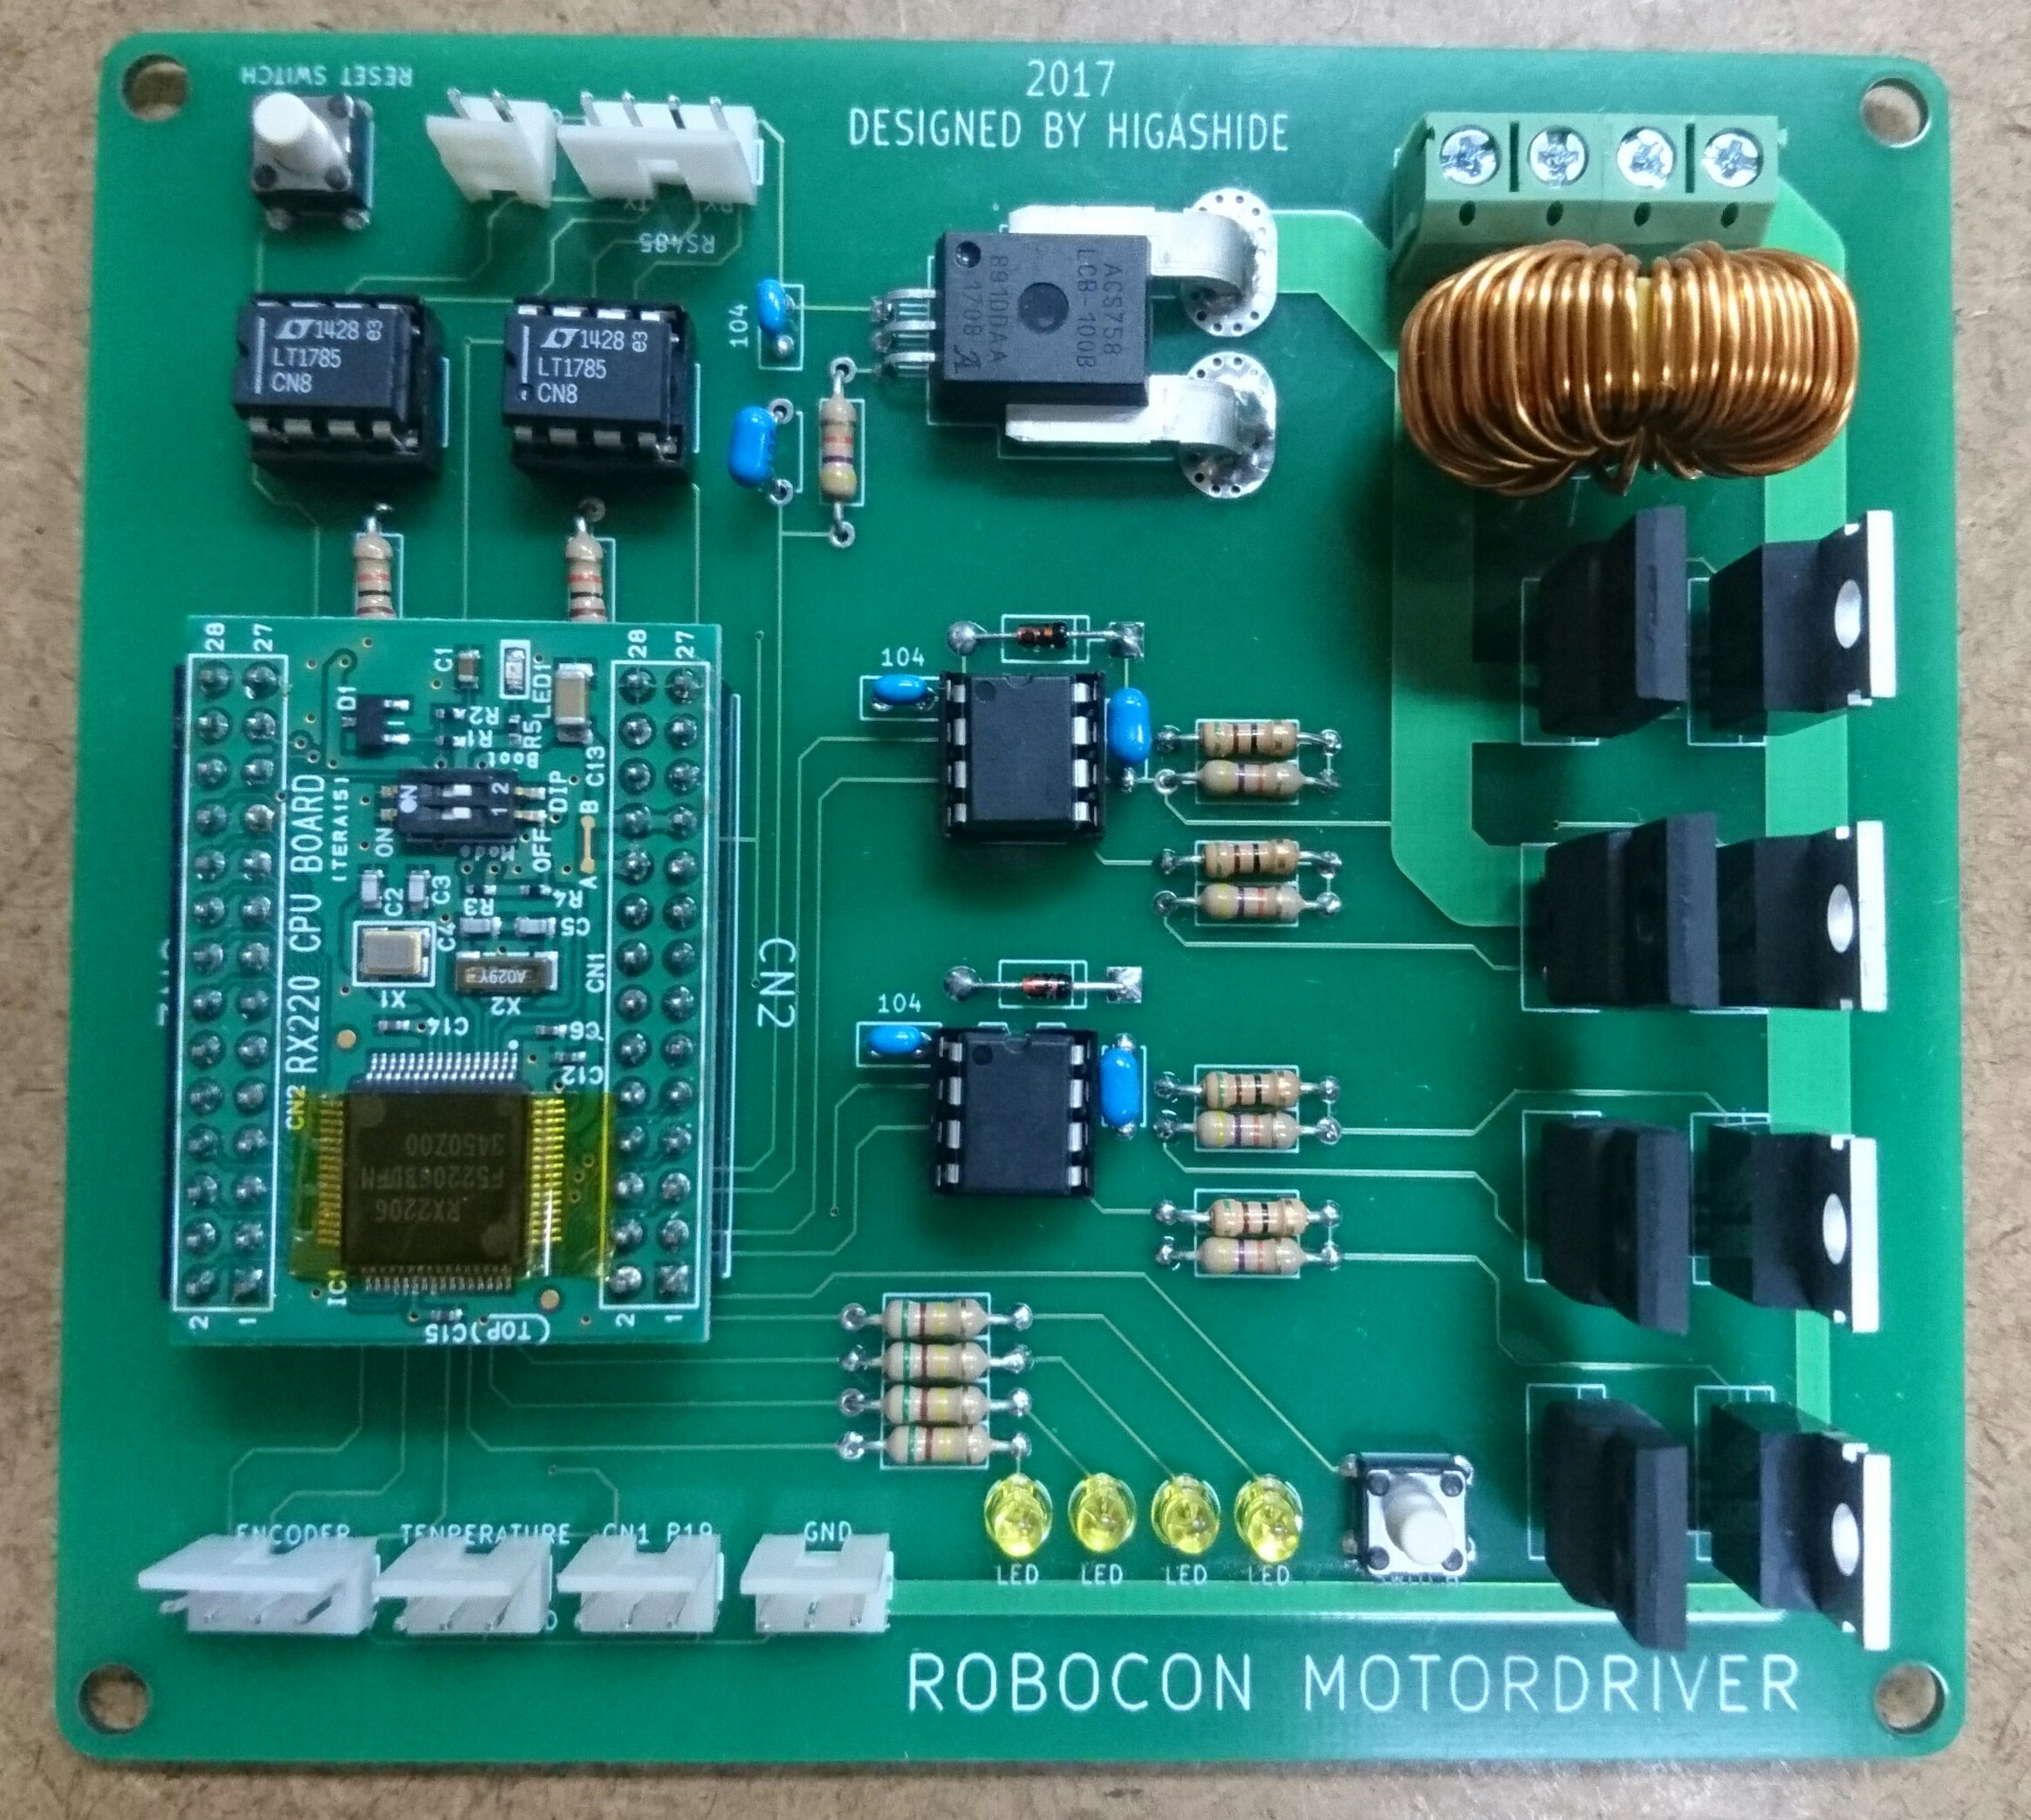
\includegraphics[width=150mm]{kankumi}
\end{center}
\caption{組み付け後}
\label{fig:kankumi}
\end{figure}

\section{実機の動作実験}
動作の確認として以下の実験を行った.
\begin{itemize}
\item LEDが点灯するか
\item 汎用スイッチが動作するか
\item リセットスイッチでRXマイコンのリセットが可能か
\item RXマイコンからPWM信号の出力が可能か
\end{itemize}

\section{実験結果}
実験の結果,以下のようになった.
\begin{itemize}
\item 図\ref{fig:jikken}のように,LEDの点灯を確認
\item 汎用スイッチ動作を確認
\item リセットスイッチでリセット確認
\item PWM信号の出力により,モータが回転することを確認
\end{itemize}
\begin{figure}[H]
\begin{center}
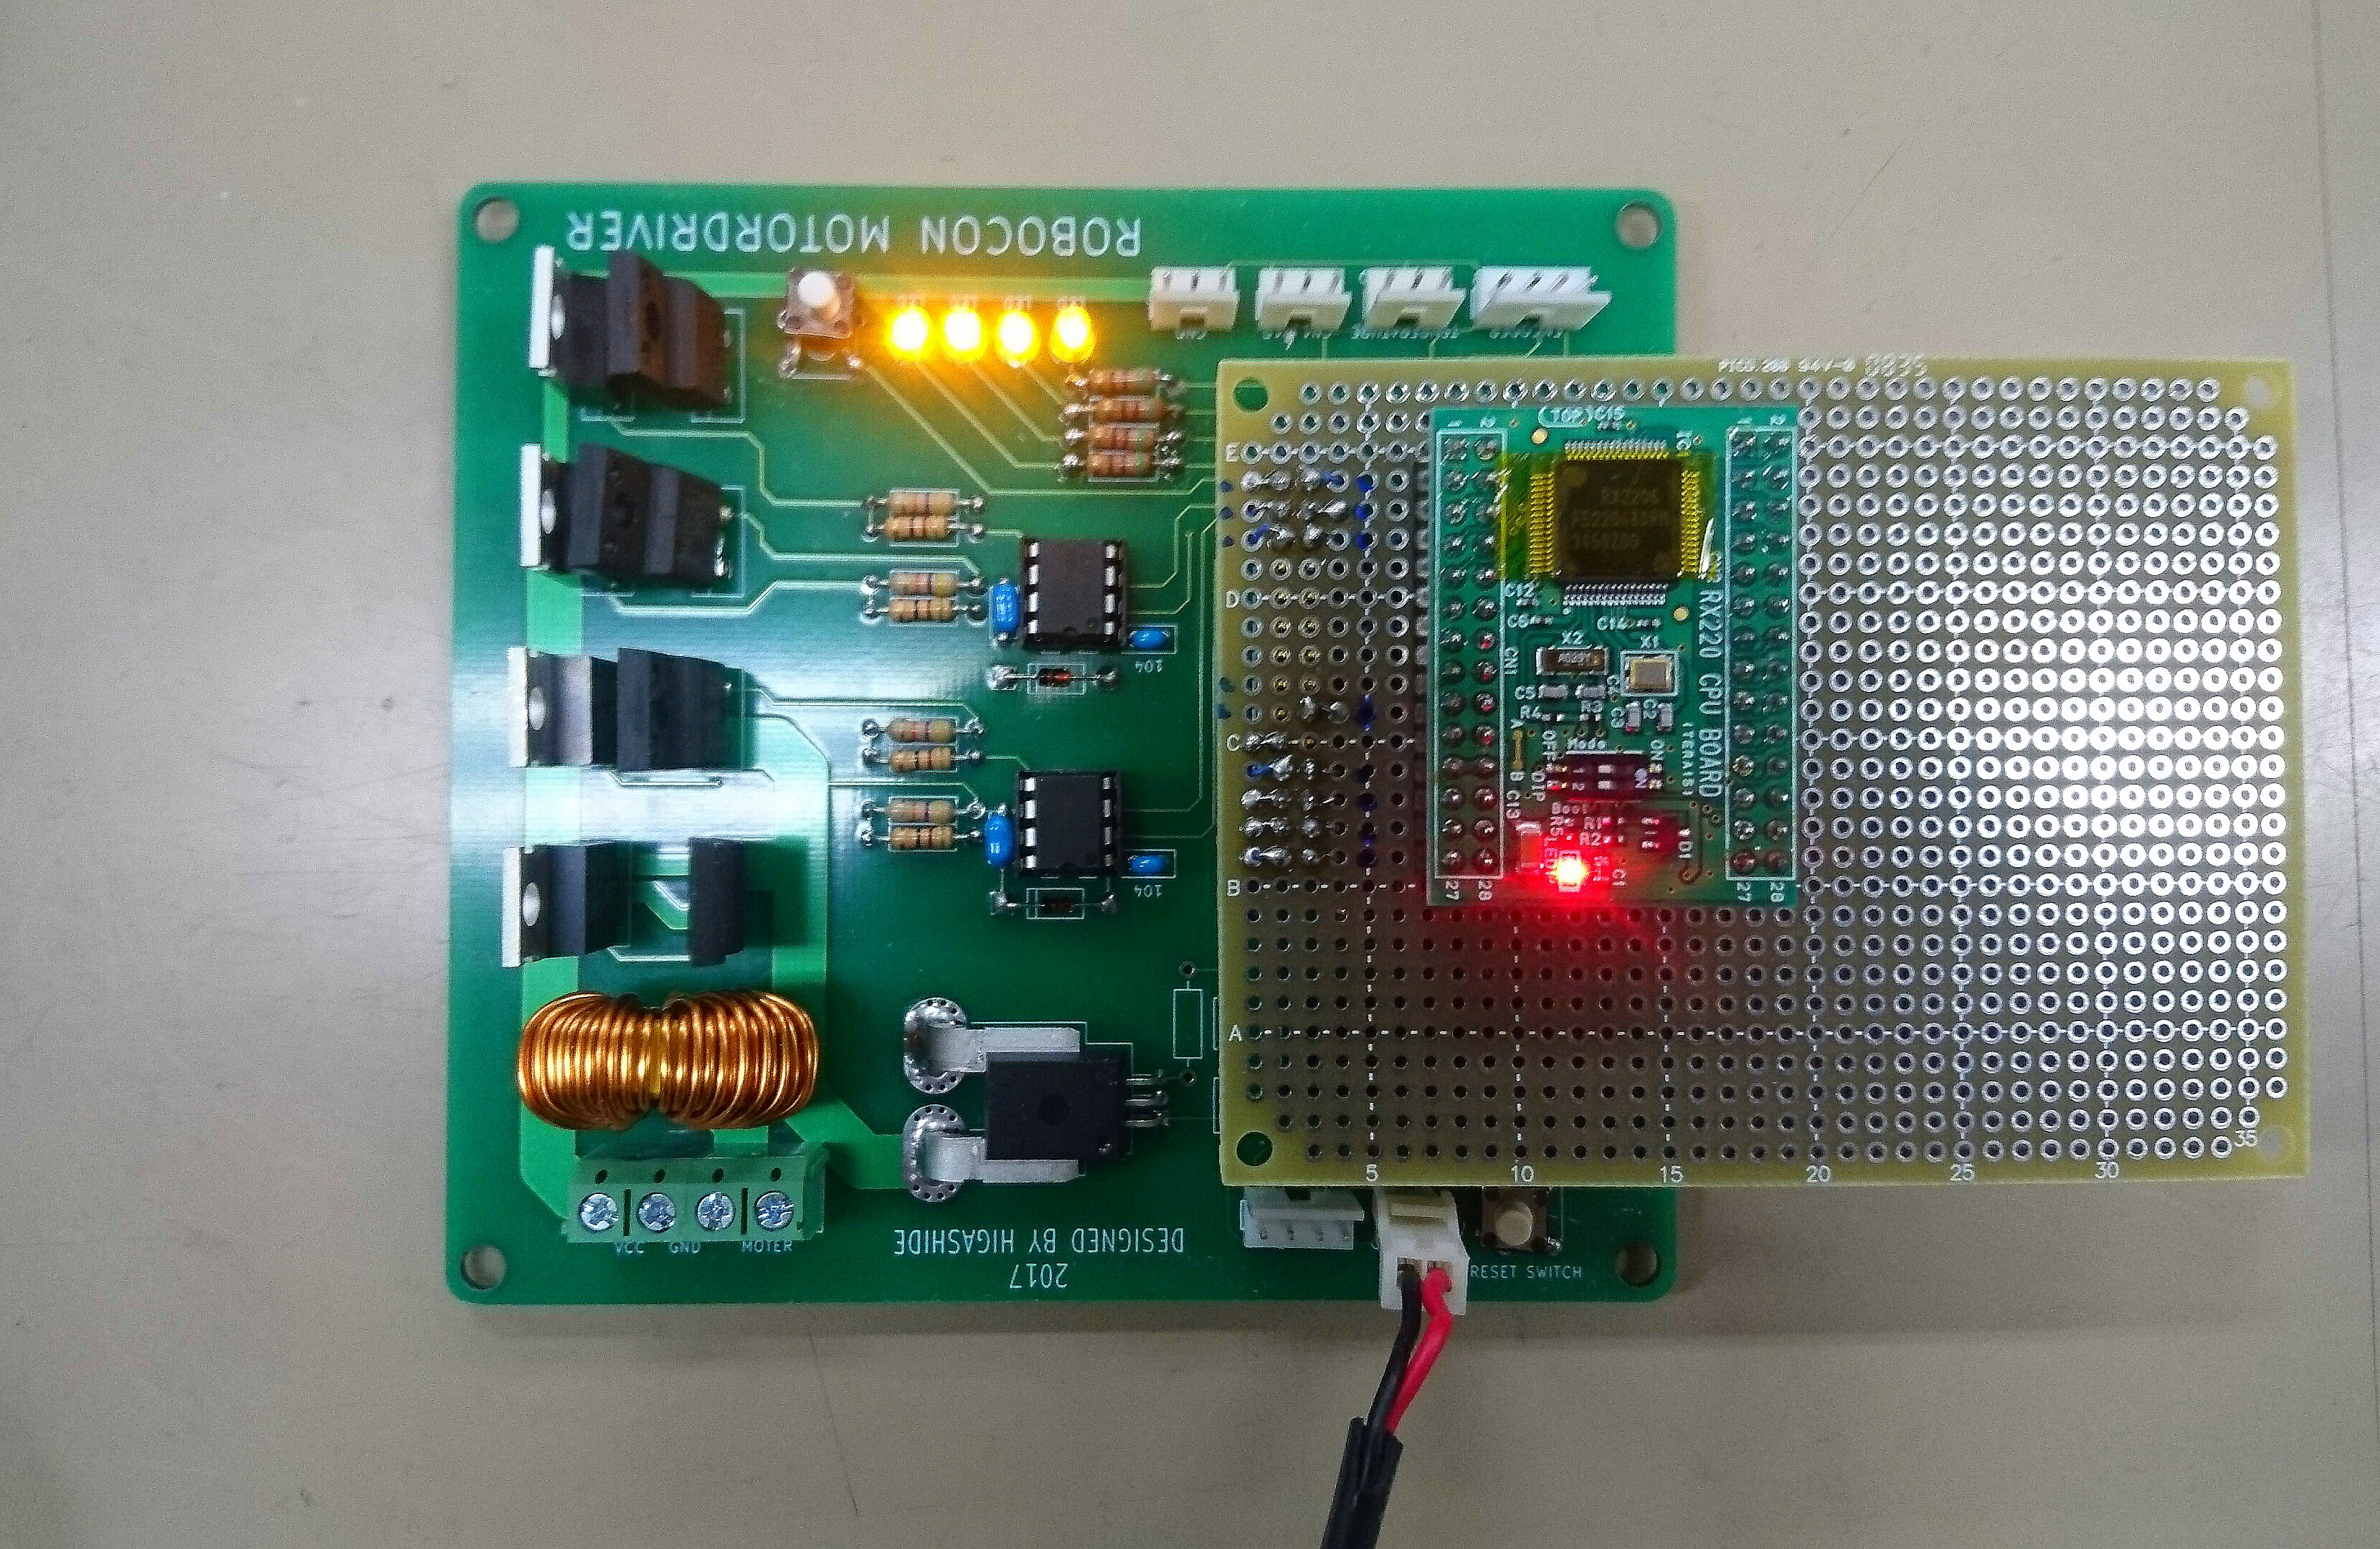
\includegraphics[width=140mm]{jikken}
\end{center}
\caption{LEDの点灯している高出力モータドライバ}
\label{fig:jikken}
\end{figure}

\section{考察}
以上の結果から,配線の間違いはないことが分かる.
また,モータが回転したことから,RXマイコンのPWM信号でハーフブリッジドライバ,FETが問題
なく機能していることが分かる.


\chapter{おわりに}
既存のITOLAB MOTORDRIVERを基に改良することで,短期間でモータドライバを製作すること
ができた.
また,KiCadを用いることで,設計時間の短縮ができた.

今後,電流センサ,温度センサの検出値の確認,RXマイコンによるシリアル通信の確認が必要
である.







\chapter*{謝辞}
\addcontentsline{toc}{chapter}{謝辞}
ロボット作成時に,知識の少ない電気分野を丁寧にご指導,サポートして下さった林道大教授,
ロボット作成時に,予定が遅れていた時に喝を入れて下さったり本論文作成にあたり研究の考
え方,方法のまとめ方などご指導,ご鞭撻していただいた伊藤恒平教授に厚く御礼申し上げます.

特に回路作成時に指導していただいたり,不得意なプログラムを助けて頂いた林道大教授に大変
ご苦労をかけてしまいましたこと心よりお詫び申し上げます.

その他,助けていただいた多くの皆様に心から感謝しております.ありがとうございました.

\appendix
\begin{thebibliography}{8}
\bibitem{hon}寺前裕司,1人で始めるプリント基板作り[完全フリーKicad付き],CQ出版株式会社,2014/7/1
\bibitem{ob} KiCADで基本設計,\url{http://www.kicad.xyz/}
\bibitem{sei} KiCad で雑に基板を作る チュートリアル,\url{https://www.slideshare.net/soburi/kicad-53622272}
\end{thebibliography}





\chapter{ITOLABMOTORDRIVER 電子部品リスト}
\begin{tabular}{|c|c|c|c|} \hline
 &部品名&型番&PDF URL\\ \hline
 1&4P,EIコネクタピンヘッダ&171825-4-50P&\url{https://jp.misumi-ec.com/}\\
 &                       &            &\url{pdf/el/2015_H/0380.pdf}\\ \hline
2&回生ダイオード&20ETS12FP&\url{http://akizukidenshi.com/}\\
 &              &         &\url{download/ds/vishay/}\\
 &              &         &\url{vs20ets.pdf}\\ \hline
3&ターミナルブロック&P-02333&\url{http://akizukidenshi.com/}\\
 &                  &       &\url{download/ds/alphaplus/TB}\\
 &                  &       &\url{111-2-x-x-x-x.pdf}\\ \hline
4&カーボン被膜抵抗&R-25103&\url{http://akizukidenshi.com/}\\
 &10kΩ&       &\url{download/ds/faithful/}\\
 &     &       &\url{R1_CF.pdf}\\ \hline
5&カーボン被膜抵抗&R-25103&\url{http://akizukidenshi.com/}\\
 &47kΩ&       &\url{download/ds/faithful/}\\
 &     &       &\url{R1_CF.pdf}\\ \hline
6&カーボン被膜抵抗&R-25470&\url{http://akizukidenshi.com/}\\
 &47Ω&       &\url{download/ds/faithful/}\\
 &    &       &\url{R1_CF.pdf}\\ \hline
7&汎用小信号高速&1N4148&\url{http://akizukidenshi.com/}\\
 &スイッチング・ダイオード&      &\url{download/1n4148.pdf}\\ \hline
8&セラミックコンデンサ&P-00090&\url{http://akizukidenshi.com/}\\
 &0.1μ&       &\url{download/ds/murata/}\\
 &     &       &\url{RPEF11H104Z2P1A01B_a.pdf}\\ \hline
9&セラミックコンデンサ&P-03095&\url{http://akizukidenshi.com/}\\
 &10μ&        &\url{download/rd_series.pdf}\\ \hline
\end{tabular}
\begin{tabular}{|c|c|c|c|} \hline
10&ハーフブリッジドライバ&IR2302PBF&\url{http://akizukidenshi.com/}\\
  &8-DIP&    &\url{download/ds/ir/ir2302.pdf}\\ \hline
11&ピンソケット&c-03951&\url{http://akizukidenshi.com/}\\
  &14×2P&    &\url{download/ds/kakusya/}\\
  &      &    &\url{FH-2X00SG.pdf}\\ \hline
12&RX200マイコンボード&K-08769&\url{http://akizukidenshi.com/}\\
  &                   &       &\url{download/ds/akizuki/}\\
  &                   &       &\url{RX220_CPU_Manual.pdf}\\ \hline
13&トロイダルコイル&P-06731&\url{http://akizukidenshi.com/}\\
  &330μH9A&     &\url{download/ds/core/}\\
  &        &     &\url{TCV-331M-9A-8026.pdf}\\ \hline
14&NchパワーMOSFET&EKI04047&\url{http://akizukidenshi.com/}\\
  &               &        &\url{download/ds/sanken/}\\
  &               &        &\url{eki04047_ds_en.pdf}\\ \hline
\end{tabular}

\chapter{新高出力モータドライバ 電子部品リスト}
\begin{tabular}{|c|c|c|c|} \hline
 &部品名&型番&PDF URL\\ \hline
 1&4P,EIコネクタピンヘッダ&171825-4-50P&\url{https://jp.misumi-ec.com/}\\
 &                       &            &\url{pdf/el/2015_H/0380.pdf}\\ \hline
2&回生ダイオード&20ETS12FP&\url{http://akizukidenshi.com/}\\
 &              &         &\url{download/ds/vishay/}\\
 &              &         &\url{vs20ets.pdf}\\ \hline
3&ターミナルブロック&P-02333&\url{http://akizukidenshi.com/}\\
 &                  &       &\url{download/ds/alphaplus/TB}\\
 &                  &       &\url{111-2-x-x-x-x.pdf}\\ \hline
4&カーボン被膜抵抗&R-25103&\url{http://akizukidenshi.com/}\\
 &10kΩ&       &\url{download/ds/faithful/}\\
 &     &       &\url{R1_CF.pdf}\\ \hline
5&カーボン被膜抵抗&R-25103&\url{http://akizukidenshi.com/}\\
 &47kΩ&       &\url{download/ds/faithful/}\\
 &     &       &\url{R1_CF.pdf}\\ \hline
6&カーボン被膜抵抗&R-25470&\url{http://akizukidenshi.com/}\\
 &47Ω&       &\url{download/ds/faithful/}\\
 &    &       &\url{R1_CF.pdf}\\ \hline
7&汎用小信号高速&1N4148&\url{http://akizukidenshi.com/}\\
 &スイッチング・ダイオード&      &\url{download/1n4148.pdf}\\ \hline
8&セラミックコンデンサ&P-00090&\url{http://akizukidenshi.com/}\\
 &0.1μ&       &\url{download/ds/murata/}\\
 &     &       &\url{RPEF11H104Z2P1A01B_a.pdf}\\ \hline
9&セラミックコンデンサ&P-03095&\url{http://akizukidenshi.com/}\\
 &10μ&        &\url{download/rd_series.pdf}\\ \hline
\end{tabular}
\begin{tabular}{|c|c|c|c|} \hline
10&ハーフブリッジドライバ&IR2302PBF&\url{http://akizukidenshi.com/}\\
  &8-DIP&    &\url{download/ds/ir/ir2302.pdf}\\ \hline
11&ピンソケット&c-03951&\url{http://akizukidenshi.com/}\\
  &14×2P&    &\url{download/ds/kakusya/}\\
  &      &    &\url{FH-2X00SG.pdf}\\ \hline
12&RX200マイコンボード&K-08769&\url{http://akizukidenshi.com/}\\
  &                   &       &\url{download/ds/akizuki/}\\
  &                   &       &\url{RX220_CPU_Manual.pdf}\\ \hline
13&トロイダルコイル&P-06731&\url{http://akizukidenshi.com/}\\
  &330μH9A&     &\url{download/ds/core/}\\
  &        &     &\url{TCV-331M-9A-8026.pdf}\\ \hline
14&NchパワーMOSFET&EKI04047&\url{http://akizukidenshi.com/}\\
  &               &        &\url{download/ds/sanken/}\\
  &               &        &\url{eki04047_ds_en.pdf}\\ \hline
15&3mm 砲弾型LED&I-09851&\url{http://akizukidenshi.com/}\\
  &             &       &\url{download/ds/lg/}\\
  &&&\url{LEBWL34A06AA00.pdf}\\ \hline
16&タクトスイッチ&TVDP01-060CB&\url{http://akizukidenshi.com/}\\
&&&\url{download/ds/cosland/}\\
&&&\url{DTS-6-V.PDF}\\ \hline
17&温度センサ&MCP9700&\url{http://akizukidenshi.com/}\\
&&&\url{download/MCP9701-ETO.pdf}\\ \hline
18&電流センサ&ACS758LCB-100B&\url{https://www.digikey.jp/}\\
&&&\url{product-detail/}\\
&&&\url{ja/allegro-microsystems-llc/}\\
&&&\url{ACS758LCB-100B-PFF-T/}\\
&&&\url{620-1321-ND/2042746}\\ \hline
19&RS485トランシーバ&LT1785CN8&\url{http://akizukidenshi.com/}\\
&&&\url{download/lt1785cn8.pdf}\\ \hline
\end{tabular}

\chapter{ロボコン用高出力モータドライバ回路図}
\newpage
\begin{figure}[H]
\begin{center}
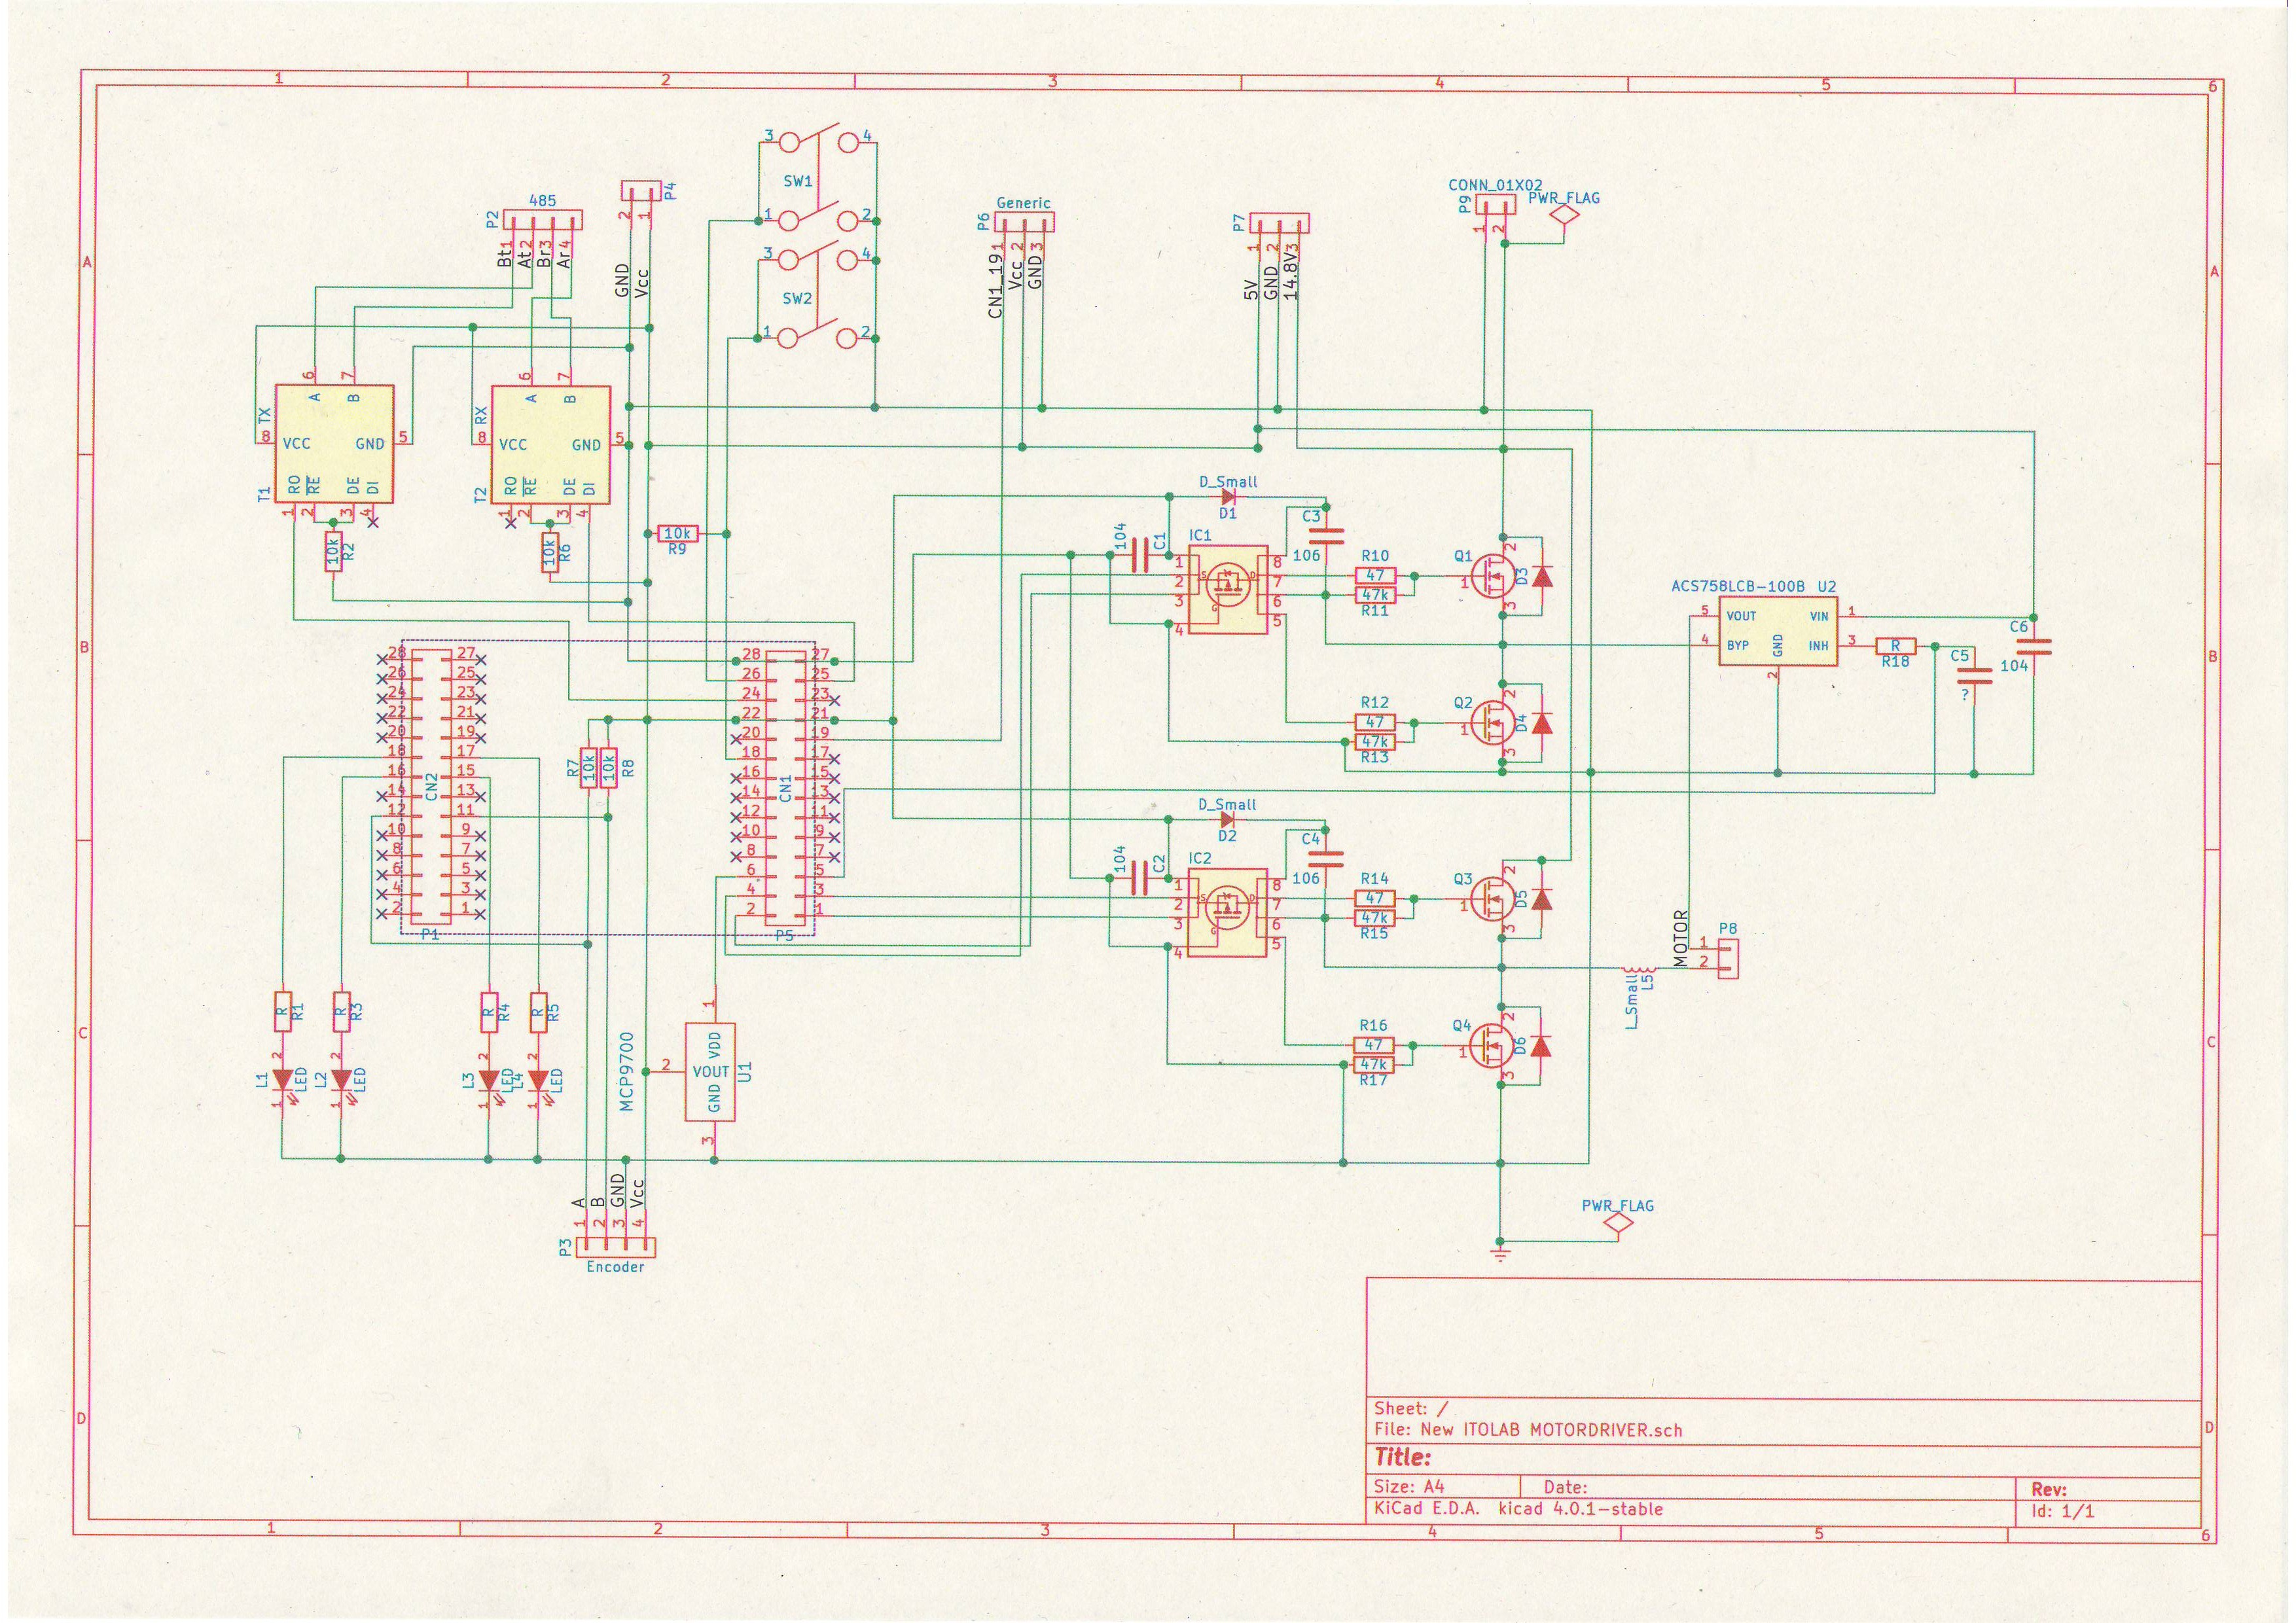
\includegraphics[width=200mm, angle=90]{kairozu2}
\end{center}
\caption{回路図}
\label{fig:kairozu2}
\end{figure}

\chapter{RXマイコンと各部品との接続}
\begin{tabular}{|c|c|c|} \hline
ピンNo.   &ポート番号&接続先           \\ \hline \hline
CN1-1     &P4-0(出力)&右ゲート ローサイド\\ \hline
CN1-2     &P4-1(出力)&左ゲート ローサイド\\ \hline
CN1-3     &P4-2(出力)&右ゲート ハイサイド\\ \hline
CN1-4     &P4-3(出力)&左ゲート ハイサイド\\ \hline
CN1-5     &P4-4(入力)&      電流センサ \\ \hline
CN1-6     &P4-6(入力)&      温度センサ \\ \hline
CN1-18    &PO-3(入力)&    汎用スイッチ \\ \hline
CN1-19    &PO-5(入力/出力)&      汎用ポート \\ \hline
CN1-21    &          &              5V \\ \hline
CN1-22    &          &              5V \\ \hline
CN1-24    &RS232(RXD)&          TX信号 \\ \hline
CN1-25    &RS232(TXD)&          RX信号 \\ \hline
CN1-26    &RES#     &リセットスイッチ \\ \hline
CN1-27    &          &             GND \\ \hline
CN1-28    &          &             GND \\ \hline \hline
CN2-11    &MTCLKA    &エンコーダB\\ \hline
CN2-12    &MTCLKB    &エンコーダA\\ \hline
CN2-15    &PH-0(出力)&汎用LED    \\ \hline
CN2-16    &PH-1(出力)&汎用LED    \\ \hline
CN2-17    &PH-2(出力)&汎用LED    \\ \hline
CN2-18    &PH-3(出力)&汎用LED    \\ \hline
\end{tabular}

\chapter{KiCadの使い方}
\begin{enumerate}
\item KiCadのホームから,図\ref{fig:1k-h}のように回路図エディタを開く.
\begin{figure}[H]
  \begin{center}
    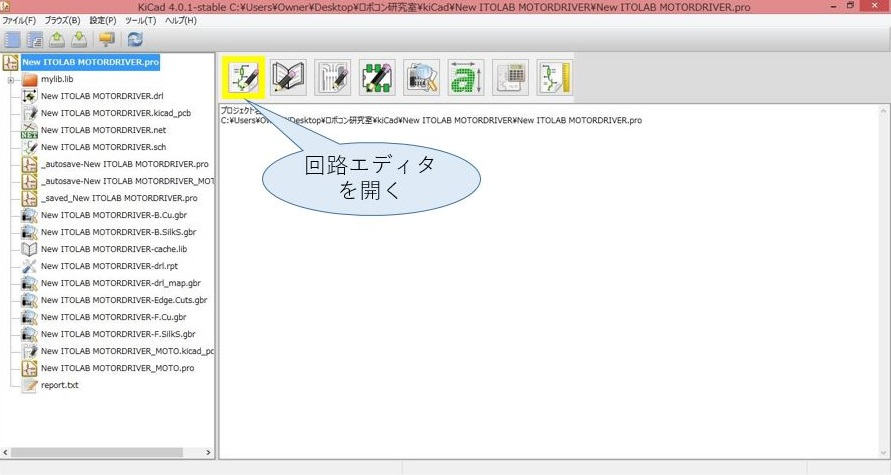
\includegraphics[width=150mm]{1k-h}
    \end{center}
  \caption{ホーム画面}
 \label{fig:1k-h}
\end{figure}
\item 回路エディタで,図\ref{fig:2k-m}のように電子部品,電源,配線を選択して回路図を
作成する.
\begin{figure}[H]
  \begin{center}
    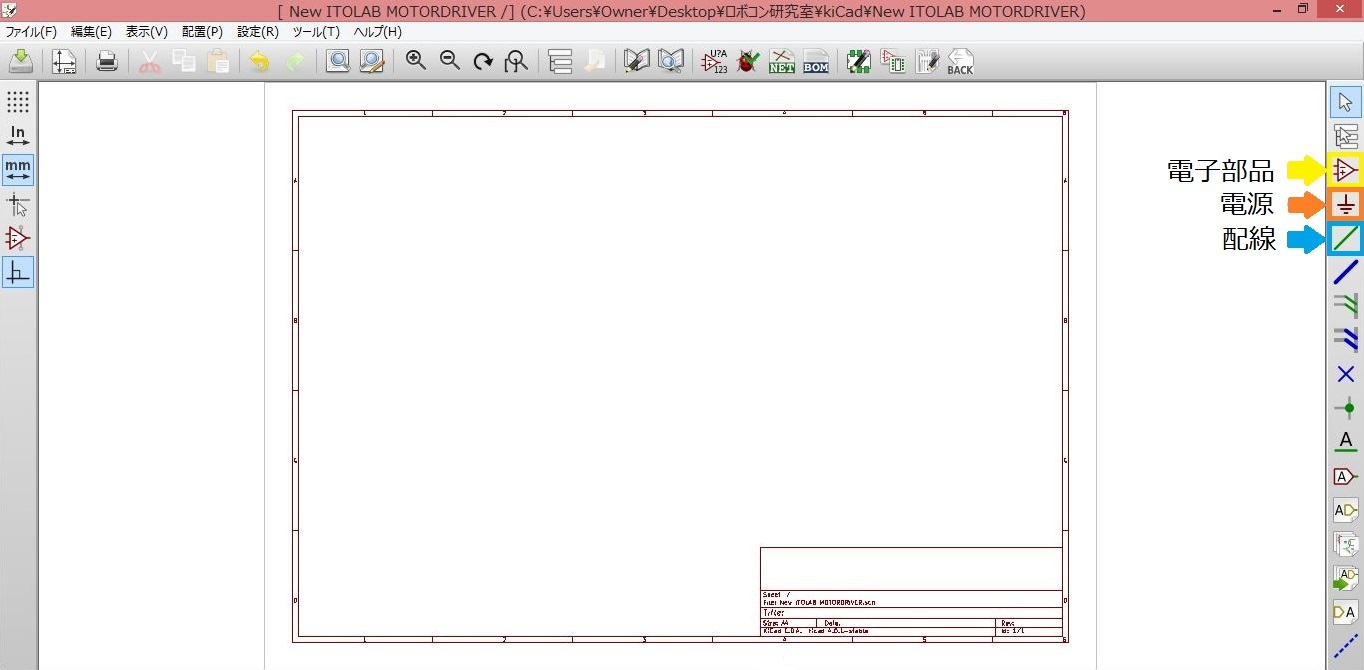
\includegraphics[width=150mm]{2k-m}
    \end{center}
  \caption{回路エディタ}
 \label{fig:2k-m}
\end{figure}
\item 回路図作成後,図\ref{fig:3m}のようにネットリストの作成を行う.
\begin{figure}[H]
  \begin{center}
    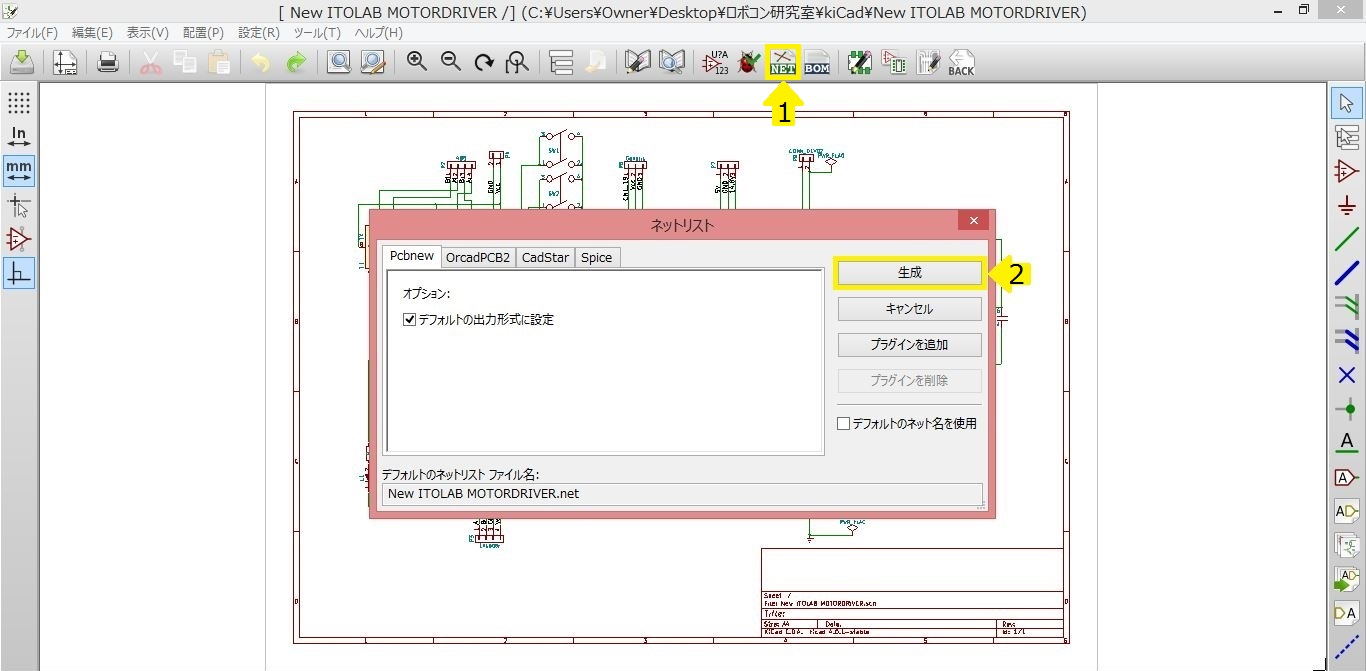
\includegraphics[width=150mm]{3m}
    \end{center}
  \caption{回路エディタ}
 \label{fig:3m}
\end{figure}
\item 図\ref{fig:4n}のようにしてコンポーネントとフットプリントの関連付けを行う.
\begin{figure}[H]
  \begin{center}
    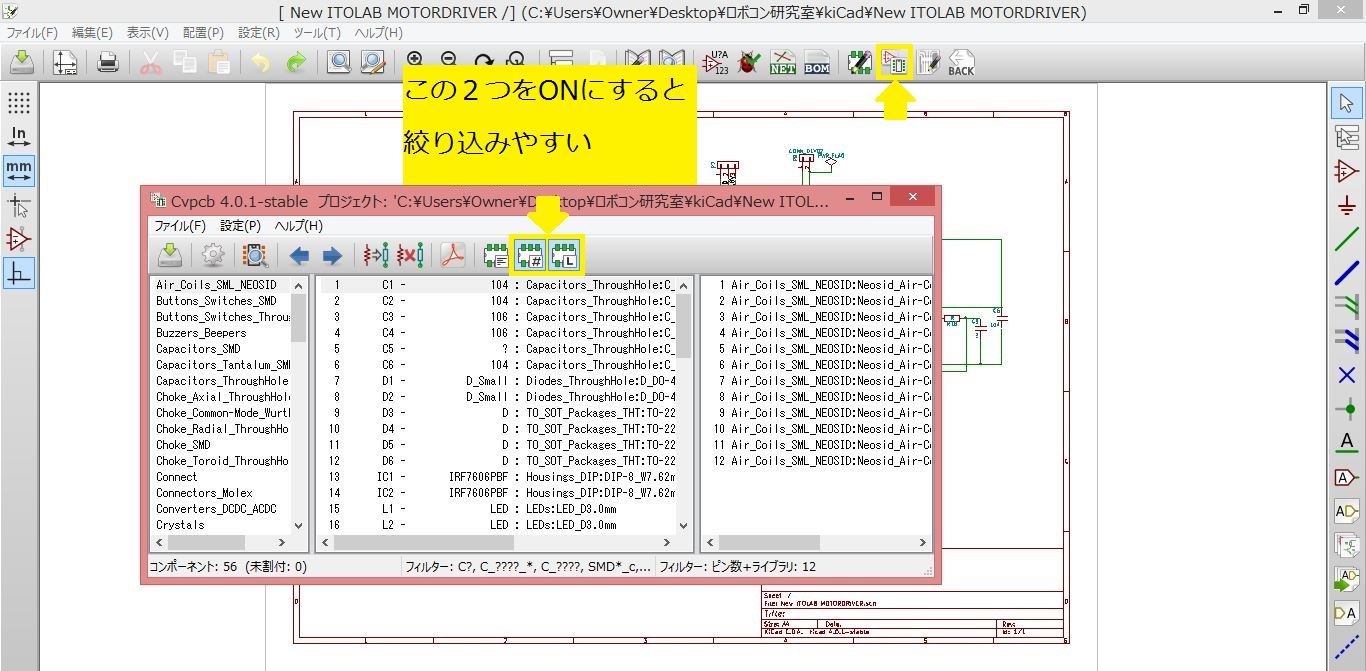
\includegraphics[width=150mm]{4n}
    \end{center}
  \caption{回路エディタ}
 \label{fig:4n}
\end{figure}
\item 図\ref{fig:5o}のように,アイコンをクリックしてプリント基板のレイアウトの
実行を行う.
\begin{figure}[H]
  \begin{center}
    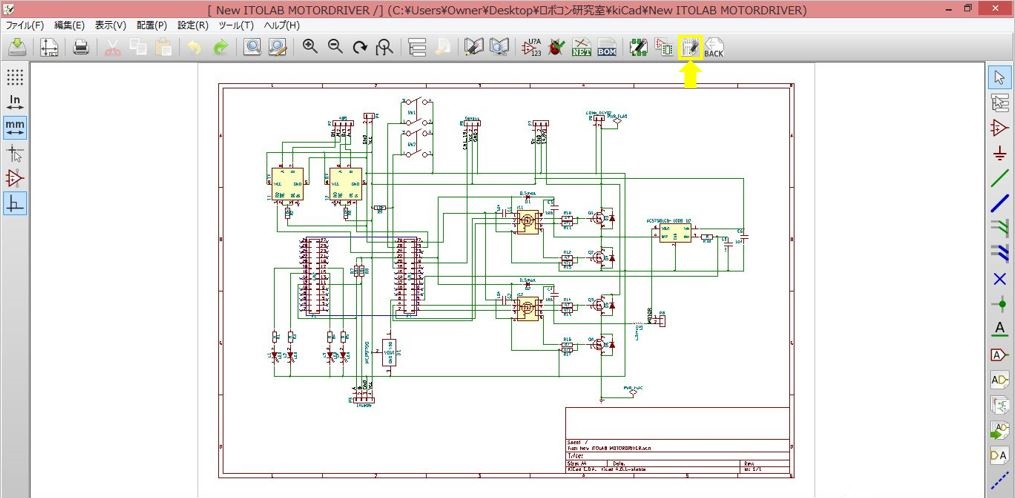
\includegraphics[width=150mm]{5o}
    \end{center}
  \caption{基板レイアウトの実行}
 \label{fig:5o}
\end{figure}
\item 図\ref{fig:6j}のようにして,ネットリストを読み込む.
\begin{figure}[H]
  \begin{center}
    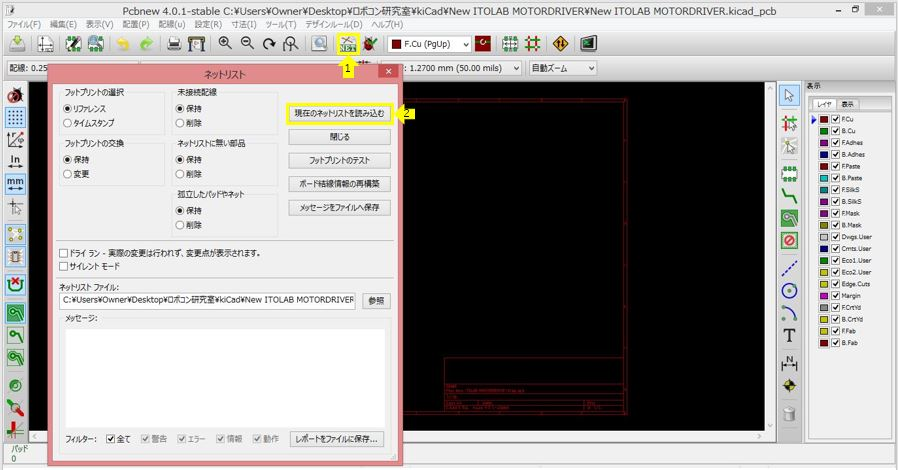
\includegraphics[width=150mm]{6j}
    \end{center}
  \caption{ネットリストの読み込み}
 \label{fig:6j}
\end{figure}
\item 図\ref{fig:7b}のように部品が表示されるので,部品をきれいに配置する.
\begin{figure}[H]
  \begin{center}
    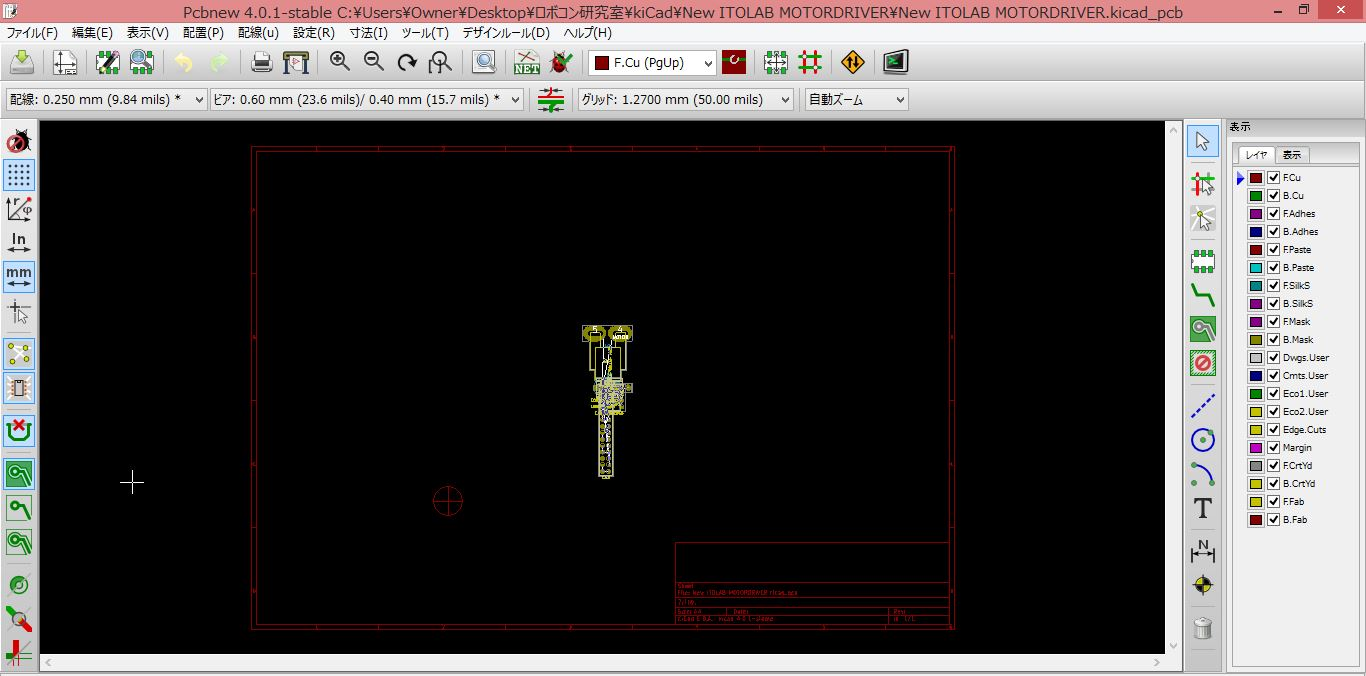
\includegraphics[width=150mm]{7b}
    \end{center}
  \caption{表示された部品}
 \label{fig:7b}
\end{figure}
\item 図\ref{fig:8b}のように,配線,基板枠の作成を行う.
\begin{figure}[H]
  \begin{center}
    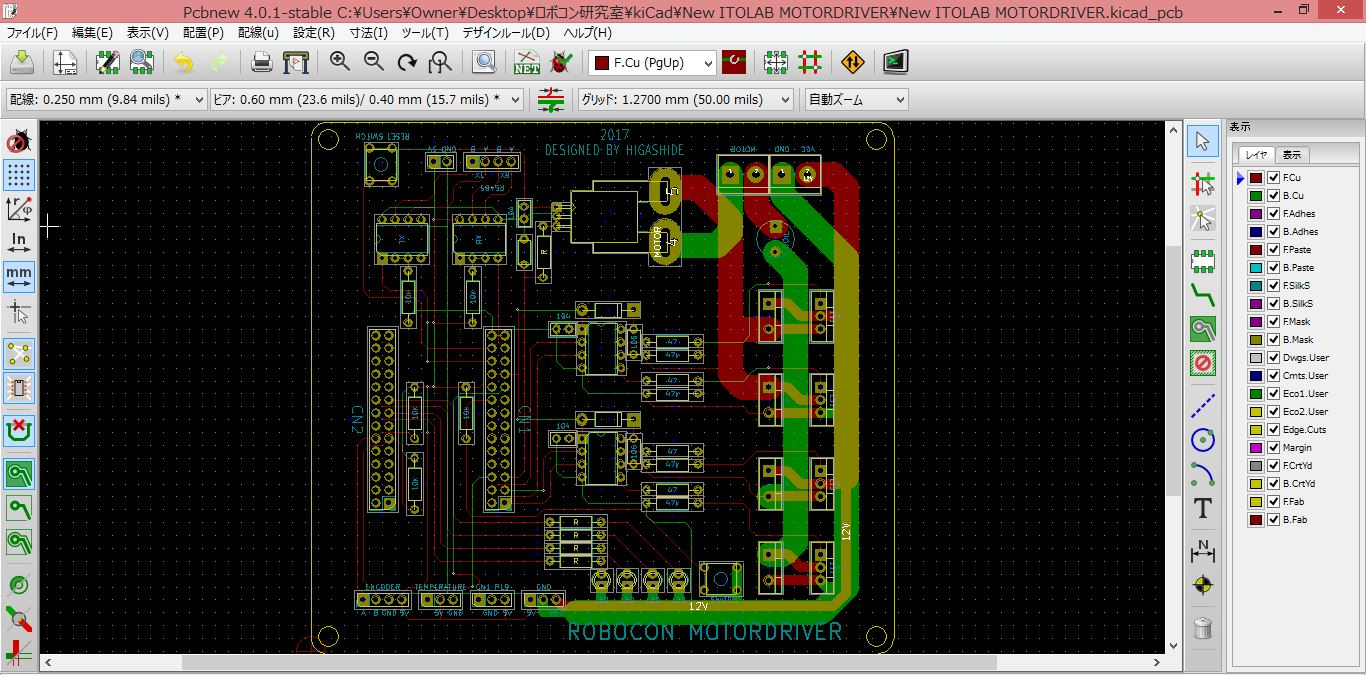
\includegraphics[width=150mm]{8b}
    \end{center}
  \caption{配線後}
 \label{fig:8b}
\end{figure}
\item 図\ref{fig:9b}のように,GNDをベタにする.
\begin{figure}[H]
  \begin{center}
    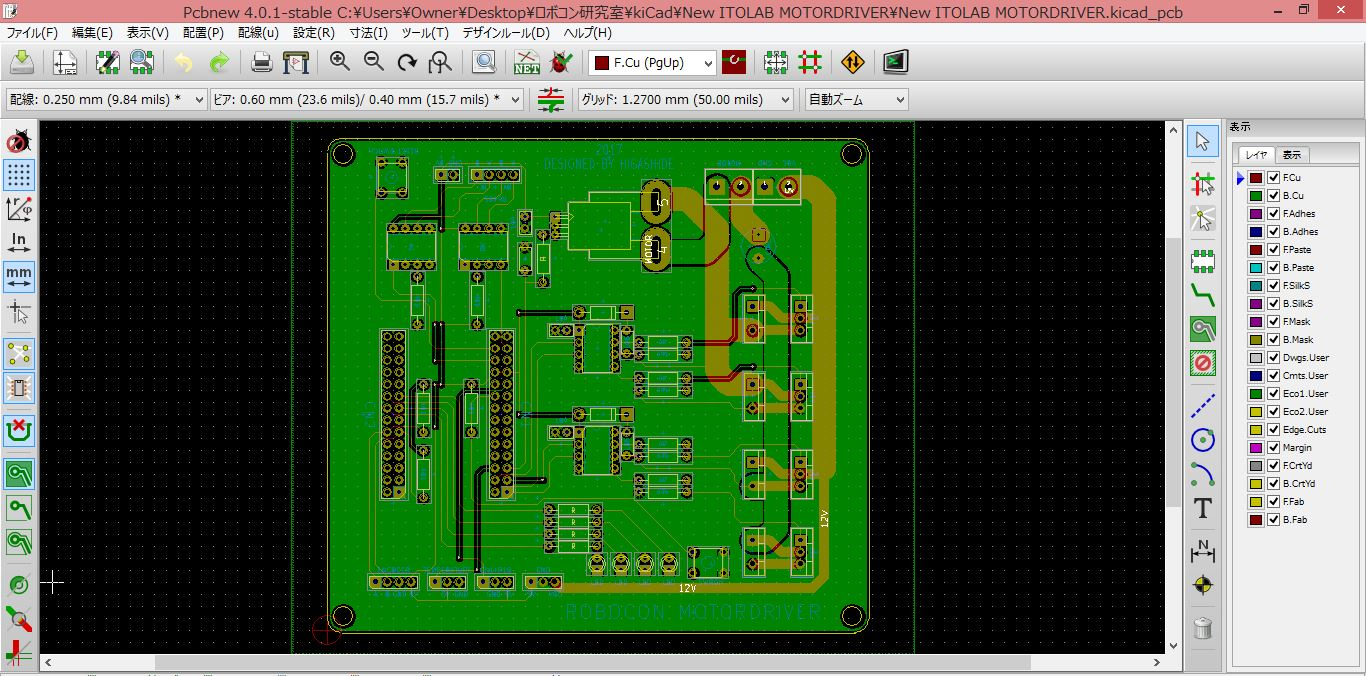
\includegraphics[width=150mm]{9b}
    \end{center}
  \caption{GNDベタ}
 \label{fig:9b}
\end{figure}
\end{enumerate}

\chapter{温度センサのデータシート}
\includepdf[pages=-]{ronbun2.pdf}
\chapter{電流センサのデータシート}
\includepdf[pages=-]{ronbun3.pdf}
\chapter{RS485トランシーバのデータシート}
\includepdf[pages=-]{ronbun4.pdf}
\chapter{FETのデータシート}
\includepdf[pages=-]{ronbun5.pdf}
\chapter{ハーフブリッジドライバのデータシート}
\includepdf[pages=-]{ronbun6.pdf}





\end{document}






